% ===========================================================================
% Arquitetura de Servidores — Infográfico Interativo
% Relatório Final — Fundamentos de Estruturas de Computadores
% Prof. Rubem Koide · Universidade Positivo · 2026.1
%
% Compilação (Overleaf ou TeX Live local):
%   pdflatex main
%   bibtex   main
%   pdflatex main
%   pdflatex main
% ===========================================================================

\documentclass[
    12pt,
    openright,
    oneside,
    a4paper,
    chapter=TITLE,
    section=TITLE,
    brazil
]{abntex2}

% ---------------------------------------------------------------------------
% PACOTES
% ---------------------------------------------------------------------------
\usepackage{lmodern}
\usepackage[T1]{fontenc}
\usepackage[utf8]{inputenc}
\usepackage{amsmath,amssymb}
\usepackage{indentfirst}
\usepackage{nomencl}
\usepackage{color}
\usepackage{graphicx}
\usepackage{microtype}
\usepackage[brazilian,hyperpageref]{backref}
\usepackage[alf]{abntex2cite}
\usepackage{booktabs}
\usepackage{longtable}
\usepackage{array}
\usepackage{xcolor}
\usepackage{listings}
\usepackage{caption}
\usepackage{tabularx}
\usepackage{hyperref}

\hypersetup{
    pdftitle={Arquitetura de Servidores — Infográfico Interativo},
    pdfauthor={Gabriel Wolff, Vitor Camillo, João Victor Alvarez, Lucas Ashikaga, Wellington Fonseca},
    pdfsubject={Fundamentos de Estruturas de Computadores},
    pdfkeywords={servidor, RAID, ECC, NUMA, virtualização, hipervisor},
    colorlinks=true,
    linkcolor=black,
    citecolor=blue,
    urlcolor=blue,
    bookmarksdepth=4
}

% ---------------------------------------------------------------------------
% LISTINGS — código embutido
% ---------------------------------------------------------------------------
\definecolor{codegray}{rgb}{0.95,0.95,0.95}
\definecolor{codekw}{rgb}{0.0,0.0,0.6}
\definecolor{codecom}{rgb}{0.0,0.5,0.0}
\definecolor{codestr}{rgb}{0.58,0.0,0.83}

\lstdefinestyle{snippet}{
    backgroundcolor=\color{codegray},
    commentstyle=\color{codecom}\itshape,
    keywordstyle=\color{codekw}\bfseries,
    stringstyle=\color{codestr},
    basicstyle=\ttfamily\footnotesize,
    breaklines=true,
    captionpos=b,
    keepspaces=true,
    showspaces=false,
    showstringspaces=false,
    showtabs=false,
    tabsize=2,
    frame=single,
    numbers=left,
    numberstyle=\tiny\color{gray},
    inputencoding=utf8,
    extendedchars=true,
    literate=%
        {á}{{\'a}}1 {à}{{\`a}}1 {ã}{{\~a}}1 {â}{{\^a}}1
        {é}{{\'e}}1 {ê}{{\^e}}1 {í}{{\'i}}1
        {ó}{{\'o}}1 {ô}{{\^o}}1 {õ}{{\~o}}1
        {ú}{{\'u}}1 {ü}{{\"u}}1
        {ç}{{\c c}}1 {Á}{{\'A}}1 {Ç}{{\c C}}1
        {ñ}{{\~n}}1 {º}{$^{\underline{o}}$}1 {ª}{$^{\underline{a}}$}1
        {—}{{---}}1 {–}{{--}}1
}
\lstset{style=snippet}

% Definição de JavaScript (não nativa no listings)
\lstdefinelanguage{JavaScript}{
    keywords={break,case,catch,continue,debugger,default,delete,do,else,false,finally,
              for,function,if,in,instanceof,new,null,return,switch,this,throw,true,try,
              typeof,var,void,while,with,const,let,async,await,yield,of,class,extends,
              super,import,export,from,Math,document,window,setTimeout},
    morecomment=[l]{//},
    morecomment=[s]{/*}{*/},
    morestring=[b]',
    morestring=[b]",
    sensitive=true
}

% ---------------------------------------------------------------------------
% DADOS DA EQUIPE E DO TRABALHO
% ---------------------------------------------------------------------------
\titulo{Arquitetura de Servidores: Infográfico Interativo \\
        \large como projeto didático para Fundamentos de Estruturas de Computadores}
\autor{Gabriel Wolff \\
       Vitor Camillo \\
       João Victor Alvarez \\
       Lucas Ashikaga \\
       Wellington Fonseca}
\local{Curitiba}
\data{Junho de 2026}
\instituicao{Universidade Positivo \par
             Escola Politécnica \par
             Disciplina de Fundamentos de Estruturas de Computadores}
\tipotrabalho{Trabalho acadêmico}
\preambulo{Trabalho final apresentado à disciplina de
           Fundamentos de Estruturas de Computadores,
           ministrada pelo Prof.\ Rubem Koide,
           Universidade Positivo, semestre 2026.1, como
           requisito parcial de avaliação.}
\orientador{Prof.\ Rubem Koide}

% ---------------------------------------------------------------------------
% INÍCIO DO DOCUMENTO
% ---------------------------------------------------------------------------
\begin{document}
\selectlanguage{brazil}
\frenchspacing

% ==================== ELEMENTOS PRÉ-TEXTUAIS ====================
\pretextual
\imprimircapa
\imprimirfolhaderosto

% ---------- RESUMO ----------
\begin{resumo}
Este trabalho apresenta o desenvolvimento de um \textbf{infográfico interativo} sobre
arquitetura de servidores como projeto didático da disciplina de Fundamentos de
Estruturas de Computadores. O artefato, escrito em HTML5, CSS3 e JavaScript ES6+
sem dependências externas, organiza-se em seis módulos navegáveis que cobrem:
(i) comparação Desktop \textit{vs.}\ Servidor com tabelas de barramentos e
interconexão multi-socket; (ii) RAID com simulador interativo de falhas,
calculadora de IOPS e aplicação da Lei de Amdahl; (iii) memória ECC e código
de Hamming \textsc{secded}; (iv) hierarquia de memória, cache associativa,
NUMA e protocolo MESI; (v) virtualização, anéis de proteção, contêineres
\textit{vs.}\ VMs e escalonadores; e (vi) síntese integrando todas as camadas
do \emph{stack} de um servidor de produção. O projeto materializa a teoria das
aulas 6 a 12 do semestre em demonstrações executáveis, com referencial
bibliográfico fundamentado em Stallings, Patterson \& Hennessy, Tanenbaum,
Silberschatz e Russinovich.

\textbf{Palavras-chave}: arquitetura de computadores; servidores; RAID;
memória ECC; NUMA; virtualização; hipervisor; infográfico interativo.
\end{resumo}

% ---------- SUMÁRIO ----------
\pdfbookmark[0]{\contentsname}{toc}
\tableofcontents*
\cleardoublepage

% ==================== ELEMENTOS TEXTUAIS ====================
\textual

\chapter{Introdução}
\label{cap:introducao}

A disciplina de \textbf{Fundamentos de Estruturas de Computadores}, ministrada pelo
Prof.\ Rubem Koide na Universidade Positivo, percorre um arco que vai dos
conjuntos numéricos e portas lógicas (aulas 2--4) até processadores
\textsc{cisc}/\textsc{risc} e sistemas operacionais (aulas 10--12),
passando pela arquitetura interna do computador e seus componentes
físicos (aulas 6--9). Em paralelo a essa progressão teórica, o curso
demanda dos alunos um projeto que materialize, em forma de artefato
didático, um recorte significativo desse conteúdo.

Este trabalho apresenta o desenvolvimento de um
\textbf{infográfico interativo sobre arquitetura de servidores},
escrito em \textsf{HTML5}, \textsf{CSS3} e \textsf{JavaScript ES6+}
sem qualquer dependência externa, executável diretamente em navegador
moderno. O recorte ``servidores'' foi escolhido por concentrar, num
único objeto de estudo, todos os subsistemas que a disciplina aborda:
do barramento e da hierarquia de memória até o escalonador de processos
e a virtualização --- portanto, exibe a teoria das aulas em ação.

\section{Justificativa}

A primeira versão do projeto, entregue em abril de 2026, recebeu como
crítica do orientador a \textit{baixa profundidade de conteúdo}: o
artefato apresentava analogias e curiosidades, mas pouca substância
técnica que se conectasse de fato com o material das aulas. Este
relatório descreve a \textbf{segunda iteração}, na qual o infográfico
foi reestruturado para incorporar:

\begin{itemize}
    \item tabelas comparativas com números reais de largura de banda,
          latência e custo (PCIe, UPI, DDR5, NVMe);
    \item fórmulas explícitas (Lei de Amdahl, cálculo de paridade
          em RAID 5, síndrome de Hamming \textsc{secded});
    \item \textit{specs} concretas de processadores citados em
          aula (Intel Core i7-5960X, Xeon Scalable, EPYC);
    \item simuladores executáveis (acesso à cache hit/miss,
          calculadora de IOPS, escalonador rubro-negro CFS); e
    \item bibliografia formal \textsc{abnt} \textsc{nbr 6023}
          com 17 referências, acessíveis diretamente da página
          via citações clicáveis.
\end{itemize}

\section{Objetivos}

\subsection{Objetivo geral}

Desenvolver um \textbf{infográfico interativo} que explique, de modo
visual e exploratório, os principais subsistemas que diferenciam um
servidor de um computador pessoal, conectando explicitamente cada
conceito ao conteúdo teórico das aulas 6--12 da disciplina.

\subsection{Objetivos específicos}

\begin{enumerate}
    \item Comparar Desktop \textit{vs.}\ Servidor em quatro dimensões
          --- alimentação, interconexão CPU--CPU, barramentos de E/S
          e gerenciamento remoto --- usando dados quantitativos.
    \item Demonstrar interativamente o comportamento de quatro
          níveis \textsc{raid} (0, 1, 5, 10) sob falha de disco e
          permitir o cálculo de capacidade útil e \textsc{iops} sob
          variação de parâmetros.
    \item Visualizar o código de Hamming \textsc{secded} usado
          em memória \textsc{ecc}, expondo a posição dos bits de
          paridade e o cálculo do síndrome.
    \item Apresentar a hierarquia de memória com latências em escala
          humana e simular a probabilidade de \textit{hit} em cada
          nível de cache.
    \item Explicar virtualização de Tipo~1 \textit{vs.}~Tipo~2,
          anéis de proteção, contêineres \textit{vs.}\ máquinas
          virtuais e o escalonador CFS do Linux.
    \item Integrar todas as camadas anteriores numa visão única do
          \textit{stack} completo de um servidor moderno.
\end{enumerate}

\section{Estrutura do trabalho}

O Capítulo~\ref{cap:referencial} estabelece o referencial teórico,
agrupado pelos seis subsistemas tratados no infográfico. O
Capítulo~\ref{cap:metodologia} descreve materiais, métodos e o
ambiente de desenvolvimento, incluindo as ferramentas de IA assistiva
empregadas. O Capítulo~\ref{cap:desenvolvimento} apresenta o
infográfico módulo a módulo, com tabelas, figuras e descrição das
simulações implementadas. O Capítulo~\ref{cap:conclusao} sintetiza os
resultados, limitações e trabalhos futuros. O Anexo~A traz o
\emph{link} do código-fonte completo no GitHub e trechos críticos do
HTML/JavaScript desenvolvido.

\chapter{Referencial Teórico}
\label{cap:referencial}

Este capítulo apresenta o referencial conceitual sobre o qual o
infográfico se apoia. As subseções a seguir espelham a estrutura
modular do artefato e estão ancoradas tanto nos livros-texto da
disciplina quanto em artigos seminais e material didático do
Prof.\ Koide~\cite{koide2026}.

\section{Desktop \textit{versus} Servidor}
\label{sec:ref-desktop-servidor}

Embora compartilhem o modelo de von Neumann~\cite{stallings2017},
desktop e servidor divergem em praticamente todos os subsistemas
físicos. Servidores exigem altíssima disponibilidade --- tipicamente
\textsc{sla} de 99,99\,\% (4,38 minutos de \textit{downtime} mensais)
ou 99,999\,\% (\textit{five-nines}, 26 segundos mensais) --- e
operação ininterrupta 24/7. Para isso adotam:

\begin{itemize}
    \item \textbf{Fontes redundantes \textit{hot-plug}} (configuração
          N+1 ou 2N), onde a queima de uma unidade não interrompe a
          operação;
    \item \textbf{Arquitetura multi-socket} (2, 4 ou 8 processadores
          numa mesma placa), com interconexão coerente ponto-a-ponto
          --- \textsc{qpi}/\textsc{upi} na Intel~\cite{intel2009qpi},
          HyperTransport/Infinity Fabric na AMD;
    \item \textbf{Memória \textsc{ecc} registrada} (\textsc{rdimm} ou
          \textsc{lrdimm}), capaz de detectar e corrigir erros de bit
          em tempo real;
    \item \textbf{Form factor padronizado em rack} EIA-310 (unidade
          básica \textsc{1u} $=$ 44,45\,mm), permitindo densidade e
          padronização em \textit{datacenters};
    \item \textbf{Gerenciamento \textit{out-of-band}} por
          microcontroladores dedicados como iDRAC (Dell), iLO (HPE)
          ou \textsc{ipmi} genérico, com endereço IP próprio e
          independente do sistema operacional principal;
    \item \textbf{Redes de alto desempenho} (10\,\textsc{gbe},
          25\,\textsc{gbe}, 100\,\textsc{gbe} ou \textsc{InfiniBand})
          com \textit{bonding} \textsc{lacp} para tolerância a
          falhas e agregação de banda.
\end{itemize}

O surgimento de cargas de trabalho de inteligência artificial
generativa redesenhou o conceito de ``servidor'' nos últimos cinco
anos. A planta passou a ser dominada por aceleradores
--- \textsc{gpu}s, \textsc{tpu}s, \textsc{npu}s --- com interconexões
dedicadas (\textsc{nv}Link, \textsc{cxl}) que ultrapassam o
\textsc{pci}e em ordens de grandeza~\cite{nvidia2023grace}.

\section{RAID --- Redundant Array of Independent Disks}
\label{sec:ref-raid}

A proposta original de Patterson, Gibson e Katz~\cite{patterson1988}
em 1988 introduziu a ideia de agrupar múltiplos discos baratos para
obter, ao mesmo tempo, desempenho e tolerância a falhas
\textit{barata}. Os principais níveis adotados na indústria são:

\begin{description}
    \item[RAID 0 (Striping)] divide blocos de dados sequencialmente
          entre $N$ discos; capacidade útil $N \cdot D$, leitura e
          escrita paralelas, \emph{zero} tolerância a falhas.
    \item[RAID 1 (Mirroring)] mantém cópia idêntica em dois discos;
          capacidade útil $D$, sobrevive à perda de $N-1$ unidades
          de um grupo espelhado.
    \item[RAID 5 (Paridade distribuída)] espalha um bloco de paridade
          $P = A \oplus B \oplus C$ entre os discos; capacidade útil
          $(N-1) \cdot D$, sobrevive à perda de \emph{um} disco,
          impõe penalidade de escrita 4$\times$ (\textit{read-modify-write}).
    \item[RAID 6] usa dois blocos de paridade independentes (P e Q);
          tolera \emph{dois} discos quebrados, com penalidade 6$\times$.
    \item[RAID 10] combina espelhamento + \textit{striping}; alta
          performance e tolerância, custa metade da capacidade bruta.
\end{description}

\subsection{Aplicação da Lei de Amdahl}

O argumento de Amdahl~\cite{amdahl1967} delimita o ganho máximo de
qualquer otimização paralela: o ganho total é limitado pela parcela
serial do trabalho. A formulação moderna em equação, derivada
posteriormente do argumento qualitativo original de 1967, expressa-se
como --- sendo $P$ a fração paralelizável do trabalho e $N$ o número
de unidades de execução:

\begin{equation}
\mathrm{Speedup}(N) = \frac{1}{(1-P) + \dfrac{P}{N}}
\label{eq:amdahl}
\end{equation}

Quando $N \to \infty$, $\mathrm{Speedup} \to 1/(1-P)$. No exemplo do
servidor \textsc{www} discutido pelo Prof.\ Koide na Aula~9
(disco 10\,000\,\textsc{rpm}, \textit{seek} médio de 8\,\textsc{ms},
páginas de 8\,\textsc{kb}), aproximadamente 99,3\,\% do tempo de
resposta é latência rotacional --- portanto serial --- e apenas 0,7\,\%
é transferência paralelizável. Substituindo na Equação~\ref{eq:amdahl}
com $P = 0{,}007$, o \textit{speedup} máximo teórico é
$1/(1-0{,}007) \approx 1{,}007\times$. Conclusão pedagógica: paralelizar
discos para esse perfil não ajuda; o vetor de otimização é
\emph{trocar a parte serial} --- substituir o \textsc{hdd} por
\textsc{ssd}.

\section{Memória ECC e o código de Hamming}
\label{sec:ref-ecc}

Em servidor 24/7, \textit{soft errors} de memória são
estatisticamente certos. Partículas subatômicas (nêutrons cósmicos
secundários e partículas $\alpha$ provenientes de contaminação de
solda) podem inverter um bit de \textsc{dram} sem aviso. O estudo
de campo de Schroeder, Pinheiro e Weber~\cite{schroeder2009},
realizado durante 2,5 anos na frota do Google, registrou taxas de
\textbf{25\,000 a 70\,000 FIT por Mbit} (erros por bilhão de
horas-dispositivo por Mbit) e mostrou que \textbf{mais de 8\,\% dos
\textsc{dimm}s} exibem ao menos um erro corrigível por ano ---
contrariando a hipótese anterior de erros raros. O estudo concluiu
ainda que os erros são predominantemente \textit{hard errors}
(defeitos de hardware), e não \textit{soft errors} transitórios.

A correção em tempo real é feita por um código corretor proposto
originalmente por Hamming~\cite{hamming1950} em 1950. Para 8 bits de
dado, o código clássico Hamming(12,8) anexa quatro bits de paridade
nas posições $2^k$ ($k=0,1,2,3$) e oferece \emph{single error
correction} (SEC). A variante \textsc{secded} (\emph{Single Error
Correction, Double Error Detection}) --- padrão em \textsc{dimm}
\textsc{ecc} registrado --- estende o código para (13,8) adicionando
um \emph{bit de paridade global}, capaz de detectar (mas não corrigir)
ocorrências de dois erros simultâneos. Cada bit de paridade cobre um
subconjunto de posições determinado por seu bit correspondente em
binário; na leitura, o controlador recalcula as paridades e obtém um
\emph{síndrome} cuja representação decimal é exatamente a posição do
bit corrompido. O hardware inverte o bit indicado e entrega o dado
correto à CPU sem qualquer participação do sistema operacional.

A norma JEDEC \textsc{jesd79-5}~\cite{jedec2025ddr5} tornou
obrigatória a presença de \textsc{ecc} \textit{on-die} na
\textsc{ddr5}, mas é importante notar: trata-se de proteção
\emph{interna} à célula, não cobrindo o \textit{datapath}
\textsc{dimm}~$\to$~CPU. Somente \textsc{rdimm}/\textsc{lrdimm} com
\textsc{ecc} de fato protegem todo o canal.

\section{Hierarquia de memória, cache e NUMA}
\label{sec:ref-hierarquia}

Patterson e Hennessy~\cite{patterson2017} formalizam o princípio:
nenhuma tecnologia de memória é simultaneamente rápida, grande e
barata. A solução é dispor camadas em pirâmide:
registradores (sub-nanossegundo) $\to$ cache L1/L2/L3
(nanossegundos) $\to$ \textsc{ram} (dezenas de nanossegundos) $\to$
\textsc{ssd} (microssegundos) $\to$ \textsc{hdd} (milissegundos).
A eficiência da pirâmide depende de duas formas de localidade:
\textbf{temporal} (dados acessados recentemente serão acessados
de novo) e \textbf{espacial} (vizinhos de um dado acessado serão
acessados em breve).

\subsection{Organização da cache}

Caches modernos são \textit{set-associative}: o endereço seleciona um
\textit{set} e a linha pode ocupar qualquer um dos $k$ \textit{ways}.
Um Intel Core i7-5960X, processador de referência citado no
material de aula~\cite{koide2026}, organiza-se assim:

\begin{center}
\begin{tabular}{lrrrr}
\toprule
Nível & Tamanho & Associatividade & Linha & Latência \\
\midrule
L1 (dados/instruções) & 32 KB     & 8-way  & 64 B & 4 ciclos \\
L2                    & 256 KB    & 8-way  & 64 B & 12 ciclos \\
L3 (\emph{LLC})       & 20 MB     & 20-way & 64 B & 38 ciclos \\
\bottomrule
\end{tabular}
\end{center}

A \textbf{linha de cache de 64 bytes} é a unidade indivisível: ler
um byte traz consigo 63 vizinhos. L1 é privada de cada \emph{core},
L3 é compartilhada por todos os \emph{cores} do mesmo \emph{socket}.

\subsection{NUMA --- Non-Uniform Memory Access}

Em servidor multi-socket, cada CPU possui seus pentes próprios de
RAM. O acesso ao banco local é rápido ($\approx 80$\,\textsc{ns}),
mas o acesso à RAM do socket vizinho passa pelo link
\textsc{upi}/Infinity Fabric e custa cerca de 140\,\textsc{ns}~\cite{stallings2017}.
Essa não-uniformidade obriga o escalonador a manter cada
\emph{thread} próxima da memória que ela toca --- conceito de
\textit{NUMA affinity} suportado por \texttt{numactl} (Linux) e
funções equivalentes da \textsc{api} Windows.

\subsection{Coerência: MESI, MESIF, MOESI}

Quando múltiplos \emph{cores} têm cópias da mesma linha de cache, é
preciso garantir consistência. O protocolo \textsc{mesi} define
quatro estados por linha: \emph{Modified, Exclusive, Shared, Invalid}.
A Intel acrescenta \emph{Forward} (\textsc{mesif}) e a AMD acrescenta
\emph{Owned} (\textsc{moesi}). Toda escrita em linha
\emph{Shared} dispara invalidações nos outros \emph{cores}; essa
operação cruza o link de coerência e custa centenas de
ciclos --- o conhecido \textit{false sharing}.

\subsection{Paginação, TLB e \textit{huge pages}}

A \textsc{mmu} traduz endereços virtuais para físicos via tabelas de
página percorridas em 4 níveis na arquitetura x86-64. A \textsc{tlb}
(\emph{Translation Lookaside Buffer}) cacheia as traduções
recentes; quando há \textit{miss}, o \textit{page walk} custa até
quatro acessos à \textsc{ram}~\cite{silberschatz2015}. Para reduzir
pressão na \textsc{tlb}, sistemas modernos suportam páginas de
2\,\textsc{mb} (\textit{huge pages}) e 1\,\textsc{gb}
(\textit{gigantic pages}), cada entrada cobrindo 512$\times$ ou
262\,144$\times$ mais memória.

\section{Virtualização e hipervisores}
\label{sec:ref-virtualizacao}

Popek e Goldberg~\cite{popek1974} estabeleceram, em 1974, três
condições para que uma arquitetura seja virtualizável:
\textbf{equivalência} (a VM deve se comportar como hardware nativo),
\textbf{eficiência} (a maior parte das instruções deve executar sem
intervenção do hipervisor) e \textbf{controle de recursos}
(o hipervisor mantém posse exclusiva dos recursos físicos). Esses
critérios não eram naturalmente satisfeitos pela arquitetura
x86 original; somente em 2005 (Intel \textsc{vt-x}) e 2006 (AMD-V) as
extensões de hardware introduziram o estado \textsc{vmx} (informalmente
chamado de Ring~$-1$) que coloca o hipervisor abaixo do
Ring~0~\cite{russinovich2017}.

\subsection{Tipo 1 \textit{vs.}\ Tipo 2}

\begin{itemize}
    \item \textbf{Tipo 1 (\textit{bare metal})}: o hipervisor é o
          próprio sistema operacional raiz, instalado diretamente
          sobre o hardware. Exemplos: VMware ESXi, KVM (kernel
          Linux + \textsc{qemu}), Hyper-V Server, Proxmox VE, Citrix
          XenServer. Performance próxima da nativa.
    \item \textbf{Tipo 2 (\textit{hosted})}: o hipervisor é um
          programa rodando sobre um sistema operacional convencional.
          Exemplos: VirtualBox (citado pelo Prof.\ Koide na Aula~12),
          VMware Workstation, Parallels Desktop. Performance reduzida
          pelo \textit{overhead} do \textsc{so} hospedeiro.
\end{itemize}

O Windows Subsystem for Linux 2 (\textsc{wsl}~2) ilustra o caso
limítrofe: é um \emph{kernel} Linux verdadeiro rodando numa VM
\textit{utility} leve gerenciada pelo Hyper-V, com \textit{boot}
quase instantâneo e integração transparente com o filesystem do
Windows via 9P.

\subsection{Contêineres: virtualização ao nível do SO}

Diferentemente da VM, o contêiner compartilha o \emph{kernel} do
\textit{host} --- isolamento é obtido por \textit{namespaces}~\cite{man7namespaces}
(PID, mount, network, IPC, UTS, user) e \textit{cgroups}~\cite{kernelcgroups}
do Linux. O resultado: \textit{boot} em $\approx
100$\,\textsc{ms}, \textit{footprint} de \textsc{mb}s, densidade
acima de 1\,000 contêineres por \emph{host}.
Orquestradores como Kubernetes escalam essa unidade para clusters de
milhares de nós.

\subsection{Escalonadores}

O \emph{Completely Fair Scheduler} (\textsc{cfs}) do Linux, introduzido
no \emph{kernel} 2.6.23 (2007), mantém todas as \texttt{task\_struct}
numa árvore rubro-negra ordenada por \texttt{vruntime} --- tempo
virtual de execução ponderado pela prioridade \emph{nice}. A cada
decisão, escolhe-se a tarefa mais à esquerda; complexidade
$\mathcal{O}(\log n)$~\cite{love2010}. O
Windows usa escalonador \emph{multilevel feedback queue} baseado em
quantum e prioridades 0--31, com a maior parte da política
implementada no \texttt{ntoskrnl.exe}~\cite{russinovich2017}.

\section{Síntese: \textit{stack} completo do servidor}
\label{sec:ref-stack}

Os cinco subsistemas anteriores não são compartimentos isolados.
Numa requisição HTTP simples a um \textit{e-commerce}, todos eles
participam: o \textit{load balancer} entrega o pacote pela rede
(camada~\ref{sec:ref-desktop-servidor}); o \textit{ingress
controller} no Kubernetes despacha para um \emph{pod}
(virtualização, \ref{sec:ref-virtualizacao}); o processo executa em
v\textsc{cpu}s mapeados em \emph{cores} físicos com afinidade
\textsc{numa} (\ref{sec:ref-hierarquia}); buffers são alocados em
\textsc{ram} \textsc{ecc} (\ref{sec:ref-ecc}); páginas são lidas de
um \textsc{ssd} integrado a \textsc{raid}~10 (\ref{sec:ref-raid}); e
a resposta retorna percorrendo a mesma cadeia em sentido inverso.

A última seção do infográfico, descrita no
Capítulo~\ref{cap:desenvolvimento}, materializa essa visão
integradora.

\chapter{Materiais e Métodos}
\label{cap:metodologia}

Este capítulo descreve o ambiente físico, as ferramentas de software,
a abordagem metodológica e a divisão de responsabilidades adotadas
durante o desenvolvimento do infográfico.

\section{Hardware utilizado no desenvolvimento}
\label{sec:hardware}

O artefato foi desenvolvido em um \textbf{notebook Acer Aspire A315-42}
com configuração de uso típico de aluno de graduação, conforme
detalhado na Tabela~\ref{tab:hw}.

\begin{table}[h!]
\centering
\caption{Especificações do equipamento de desenvolvimento}
\label{tab:hw}
\begin{tabular}{lp{8.5cm}}
\toprule
\textbf{Componente} & \textbf{Especificação} \\
\midrule
Processador & AMD Ryzen 5 3500U, 4 \emph{cores} físicos / 8
              \emph{threads}, 2,1\,\textsc{ghz} base \\
Arquitetura  & x86\_64, AMD Zen+, fabricação 12\,\textsc{nm} \\
Memória RAM  & 9,6\,\textsc{gib} \textsc{ddr4} 2400\,\textsc{mhz}
               (não-\textsc{ecc}, conforme classe consumidor) \\
Armazenamento & SSD \textsc{nvme} M.2, 512\,\textsc{gb} \\
Sistema operacional & EndeavourOS (base Arch Linux),
                      \emph{kernel} 7.0.9-zen1 \\
Navegador alvo & Chromium 134+, Mozilla Firefox 130+ \\
\bottomrule
\end{tabular}
\end{table}

Por se tratar de aplicação web client-side, o infográfico foi
testado também em equipamentos diversos dos demais integrantes da
equipe, com sistemas operacionais Windows~11 e macOS~14, confirmando
compatibilidade transversal nos navegadores baseados em Chromium e
no Mozilla Firefox.

\section{Ferramentas e ambiente de desenvolvimento}
\label{sec:ferramentas}

\subsection{Editor de código}

O desenvolvimento foi conduzido no \textbf{Visual Studio Code}
\cite{vscode2026}, distribuído pela Microsoft sob licença
\textsc{mit}. As extensões utilizadas restringiram-se ao conjunto
mínimo necessário: \textit{Prettier} para formatação consistente,
\textit{Live Server} para auto-reload durante o desenvolvimento e
\textit{GitLens} para visualização do histórico de commits.

\subsection{Assistentes de IA generativa}

A produção utilizou duas ferramentas de IA, declaradas conforme a
boa prática acadêmica atual de transparência sobre uso de modelos
generativos:

\begin{description}
    \item[Google Gemini --- modo Canvas~\cite{gemini2026}.] Empregado
          na fase inicial de prototipagem, especialmente na geração
          de andaime visual em HTML/CSS para os módulos
          interativos (estrutura inicial do simulador \textsc{raid} e
          das barras de recursos da virtualização).
    \item[Anthropic Claude Code~\cite{claudecode2026}.] Empregado na
          segunda iteração para aprofundamento técnico do conteúdo,
          refatoração da disposição em sub-abas, escrita das tabelas
          comparativas, redação deste relatório e elaboração do
          roteiro de defesa. A interação se deu via terminal sobre
          o diretório do projeto, com revisão humana de cada commit.
\end{description}

Ambas as ferramentas atuaram como copiloto: o discernimento técnico,
a verificação dos números citados e a aderência ao material da
disciplina foram conduzidos pelos integrantes da equipe.

\subsection{Versionamento e hospedagem}

O código-fonte está versionado em \textsf{Git} e hospedado no
GitHub no repositório
\url{https://github.com/glkwolff/Projeto-Estruturas-de-computadores}.

\subsection{Stack tecnológico do artefato}

O infográfico final é \emph{auto-contido}: um único arquivo
\texttt{projeto.html} (\textasciitilde 2.500 linhas) contendo
estrutura, estilos e lógica. Não há \emph{build step}, transpilação
ou dependência de pacotes externos. A Tabela~\ref{tab:stack} resume.

\begin{table}[h!]
\centering
\caption{Tecnologias usadas no artefato final}
\label{tab:stack}
\begin{tabular}{lp{8cm}}
\toprule
\textbf{Tecnologia} & \textbf{Uso} \\
\midrule
HTML5            & Estrutura semântica em \texttt{section}/
                   \texttt{article}, \texttt{table} \\
CSS3             & \emph{Custom properties}, \texttt{grid},
                   \texttt{flex}, \texttt{clip-path}, transições,
                   \emph{media queries} \\
JavaScript ES6+  & Manipulação de DOM, lógica de estado em
                   variáveis-módulo, \texttt{setTimeout} para
                   animações, \texttt{const}/\texttt{let} \\
SVG inline       & (Não utilizado --- toda visualização é
                   feita por divs estilizadas, para reduzir
                   dependência) \\
\bottomrule
\end{tabular}
\end{table}

A escolha de \emph{vanilla} JavaScript --- sem frameworks como React
ou Vue --- foi deliberada: o objetivo pedagógico é exibir conceitos
de arquitetura, não exercitar engenharia de \emph{front-end}.
Manter o projeto em arquivo único também simplifica entrega,
avaliação e execução: basta abrir o HTML no navegador.

\section{Metodologia de desenvolvimento}
\label{sec:metodologia-dev}

O projeto seguiu duas iterações sucessivas:

\begin{enumerate}
    \item \textbf{Iteração 1 (abril/2026)}. Versão inicial entregue
          como parcial, focada em estabelecer o esqueleto visual e os
          cinco módulos básicos com analogias e curiosidades. Avaliada
          como insuficientemente profunda pelo orientador.
    \item \textbf{Iteração 2 (junho/2026)}. Refatoração com foco em
          \emph{profundidade conteudística}: incorporação de tabelas
          quantitativas, fórmulas explícitas, simuladores adicionais
          (calculadora \textsc{raid}, simulador de cache hit/miss,
          escalonador rubro-negro), reorganização de cada módulo em
          sub-abas para reduzir densidade visual e adição de um
          sexto módulo (\textit{stack} completo) integrador.
\end{enumerate}

A metodologia em cada módulo seguiu o ciclo:

\begin{enumerate}
    \item leitura do material das aulas correspondente
          (aulas 6 a 12);
    \item mapeamento dos conceitos para subseções navegáveis;
    \item definição de uma interação central ---
          ``o que o aluno pode \emph{fazer} aqui?'' ---
          em vez de ler texto passivo;
    \item implementação progressiva, testando hot-reload no
          navegador;
    \item revisão pela equipe e ajuste fino.
\end{enumerate}

\section{Divisão de responsabilidades na equipe}
\label{sec:equipe}

A equipe é composta por cinco integrantes, com divisão temática
para garantir profundidade individual em pelo menos um módulo
(condição da nota de defesa, que é individual). A
Tabela~\ref{tab:equipe} resume.

\begin{table}[h!]
\centering
\caption{Distribuição de responsabilidades por integrante}
\label{tab:equipe}
\begin{tabular}{ll}
\toprule
\textbf{Integrante} & \textbf{Módulo principal de apresentação} \\
\midrule
Gabriel Wolff       & Módulo 1 --- Desktop \textit{vs.}\ Servidor \\
Vitor Camillo       & Módulo 2 --- RAID + Lei de Amdahl \\
João Victor Alvarez & Módulo 3 --- Memória \textsc{ecc} + Hamming \\
Lucas Ashikaga      & Módulo 4 --- Hierarquia \& \textsc{numa} \\
Wellington Fonseca  & Módulo 5 --- Virtualização \\
Equipe (coletivo)   & Módulo 6 --- \emph{Stack} completo (síntese) \\
\bottomrule
\end{tabular}
\end{table}

A divisão temática não impediu colaboração em todos os módulos: cada
integrante revisou e contribuiu para os demais, mas tem domínio
aprofundado do tema que apresentará na defesa.

\section{Critérios de avaliação e entrega}

Conforme orientação do professor, a avaliação é composta de duas
notas independentes:

\begin{itemize}
    \item \textbf{Apresentação de defesa} (individual, 2,5 pontos):
          duração máxima de 15 minutos, com cada integrante
          apresentando seu módulo principal.
    \item \textbf{Relatório escrito} (coletivo, 2,5 pontos): este
          documento, com estrutura \textsc{abnt}.
\end{itemize}

A entrega final compreende um arquivo \texttt{.zip} contendo o
relatório em PDF, a apresentação, o arquivo \texttt{projeto.html} do
infográfico e o \emph{link} para o repositório GitHub (uma vez que
o código-fonte completo ultrapassa as 2\,500 linhas, conforme
preconizado pelo critério de entrega).

\chapter{Desenvolvimento e Resultados}
\label{cap:desenvolvimento}

Este capítulo descreve cada um dos seis módulos do infográfico,
apresentando: (i)~o conceito teórico que o módulo materializa,
(ii)~as sub-abas que dividem o conteúdo, (iii)~as tabelas e dados
incorporados e (iv)~as simulações interativas implementadas em
JavaScript. Reproduções das telas são apresentadas como
Figuras~\ref{fig:mod1}--\ref{fig:mod6} (capturadas em
3 de junho de 2026, navegador Firefox).

\section{Arquitetura geral do infográfico}
\label{sec:arq-geral}

O artefato organiza-se segundo uma navegação lateral com sete itens:
seis módulos temáticos mais o índice de referências bibliográficas.
Cada módulo, por sua vez, divide-se em quatro sub-abas que isolam um
recorte conceitual --- decisão de design tomada na segunda iteração
para reduzir a densidade visual percebida na primeira versão.

A Listagem~\ref{lst:nav} mostra o esqueleto de navegação:

\begin{lstlisting}[language=HTML,label=lst:nav,caption=Esqueleto da navegação lateral]
<nav>
  <button onclick="showModule('mod1', this)">Desktop vs Servidor</button>
  <button onclick="showModule('mod2', this)">RAID Interativo</button>
  <button onclick="showModule('mod3', this)">Memória ECC</button>
  <button onclick="showModule('mod4', this)">Hierarquia & NUMA</button>
  <button onclick="showModule('mod5', this)">Virtualização</button>
  <button onclick="showModule('mod6', this)">Stack Completo</button>
  <button onclick="showModule('modRef', this)">Referências</button>
</nav>
\end{lstlisting}

Internamente, cada módulo é uma \texttt{section} com
\texttt{display:none} por padrão; a função \texttt{showModule()}
ativa apenas a seção solicitada (Listagem~\ref{lst:showmodule}).

\begin{lstlisting}[language=JavaScript,label=lst:showmodule,caption=Função de navegação principal]
function showModule(modId, element) {
    document.querySelectorAll('.module').forEach(m =>
        m.classList.remove('active'));
    document.querySelectorAll('.nav-btn').forEach(b =>
        b.classList.remove('active'));
    document.getElementById(modId).classList.add('active');
    if (element) element.classList.add('active');
    window.scrollTo({ top: 0, behavior: 'smooth' });
}
\end{lstlisting}

\section{Módulo 1 --- Desktop \textit{vs.}\ Servidor}
\label{sec:mod1}

\begin{figure}[h!]
\centering
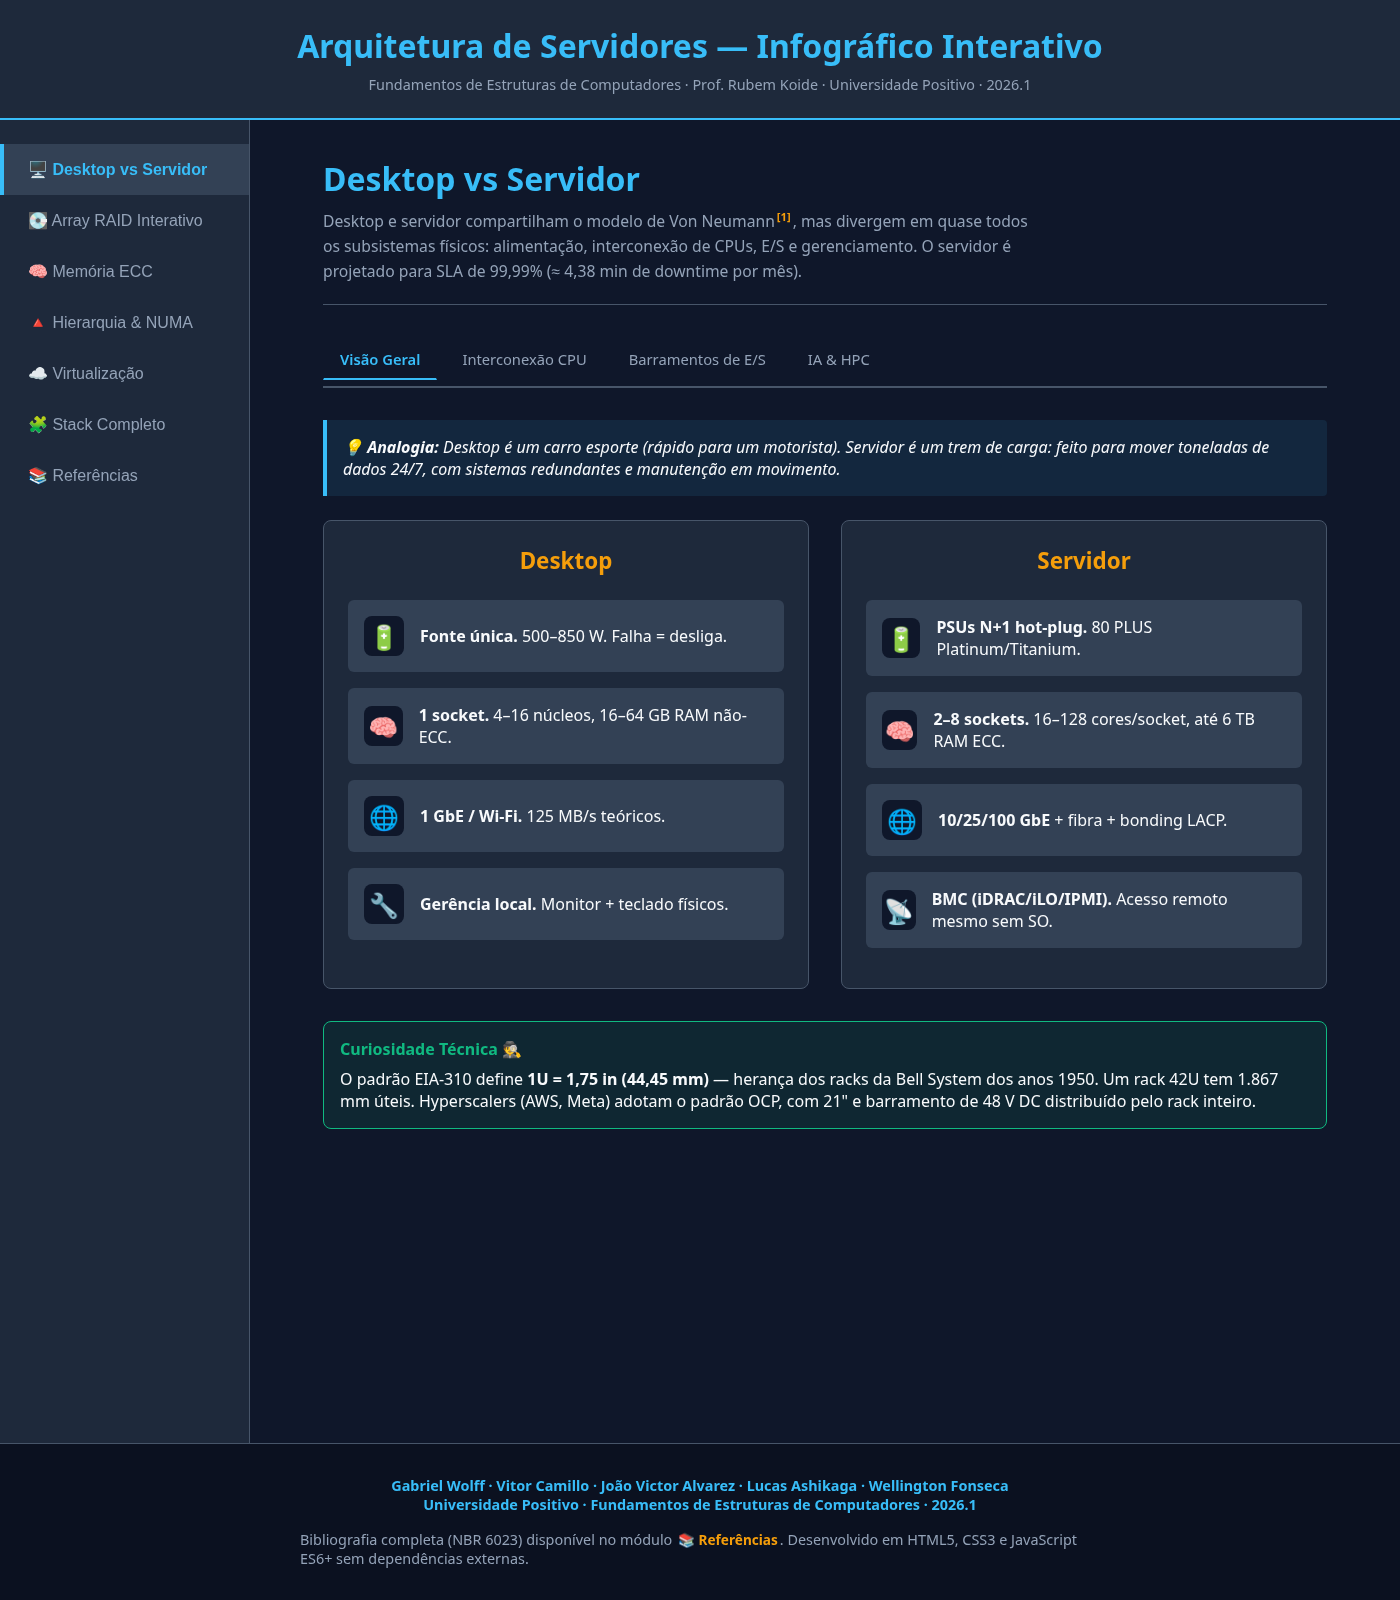
\includegraphics[width=0.95\textwidth]{figuras/mod1.png}
\caption{Módulo 1 --- Comparativo Desktop \textit{vs.}\ Servidor.}
\label{fig:mod1}
\end{figure}

O módulo apresenta quatro sub-abas:

\begin{description}
    \item[Visão Geral] grade comparativa lado-a-lado com 4 itens
          em cada coluna (alimentação, sockets, rede, gerência),
          mais analogia didática e curiosidade técnica sobre o
          padrão EIA-310.
    \item[Interconexão CPU] diagrama \emph{dual-socket} com link
          \textsc{upi} explícito (41,6\,\textsc{gb/s},
          \textasciitilde 100\,\textsc{ns}) e tabela comparativa de
          \textsc{fsb}, \textsc{qpi}, \textsc{upi}, Infinity Fabric
          e \textsc{nv}Link.
    \item[Barramentos de E/S] tabela quantitativa de
          \textsc{pci}e 3.0/4.0/5.0, \textsc{nvme}, \textsc{sata},
          1/10/100\,\textsc{gbe} e \textsc{InfiniBand}, com
          \textit{throughput} em \textsc{gb/s}.
    \item[IA \& HPC] cards com servidores de inteligência
          artificial: \textsc{nvidia} Grace Hopper GH200, AMD
          Instinct MI300X, Google TPU v5p e os supercomputadores
          \emph{El Capitan} (LLNL, nº\,1 do TOP500 desde nov/2024 com
          1,809\,\textsc{efl}\textsc{op/s}) e \emph{Frontier} (Oak
          Ridge, nº\,2 com 1,353\,\textsc{efl}\textsc{op/s}).
\end{description}

\subsection{Tabela comparativa de interconexões}

A Tabela~\ref{tab:mod1-interconexao} é a peça central da aba
``Interconexão CPU''. Os números provêm do \emph{white paper} da
Intel~\cite{intel2009qpi} e do material das aulas~\cite{koide2026}.

\begin{table}[h!]
\centering
\caption{Tecnologias de interconexão multi-socket}
\label{tab:mod1-interconexao}
\begin{tabular}{llrl}
\toprule
\textbf{Tecnologia} & \textbf{Fabricante} & \textbf{Banda} &
\textbf{Coerência} \\
\midrule
FSB             & Intel até 2008   & 10,6 GB/s  & Snooping \\
QPI             & Intel 2008--2017 & 25,6 GB/s  & MESIF (5 camadas) \\
UPI             & Intel Skylake+   & 41,6 GB/s  & MESIF + diretório \\
Infinity Fabric & AMD              & 204 GB/s   & MOESI \\
NVLink 4.0      & NVIDIA           & 900 GB/s   & GPU coherency \\
\bottomrule
\end{tabular}
\end{table}

\section{Módulo 2 --- RAID Interativo}
\label{sec:mod2}

\begin{figure}[h!]
\centering
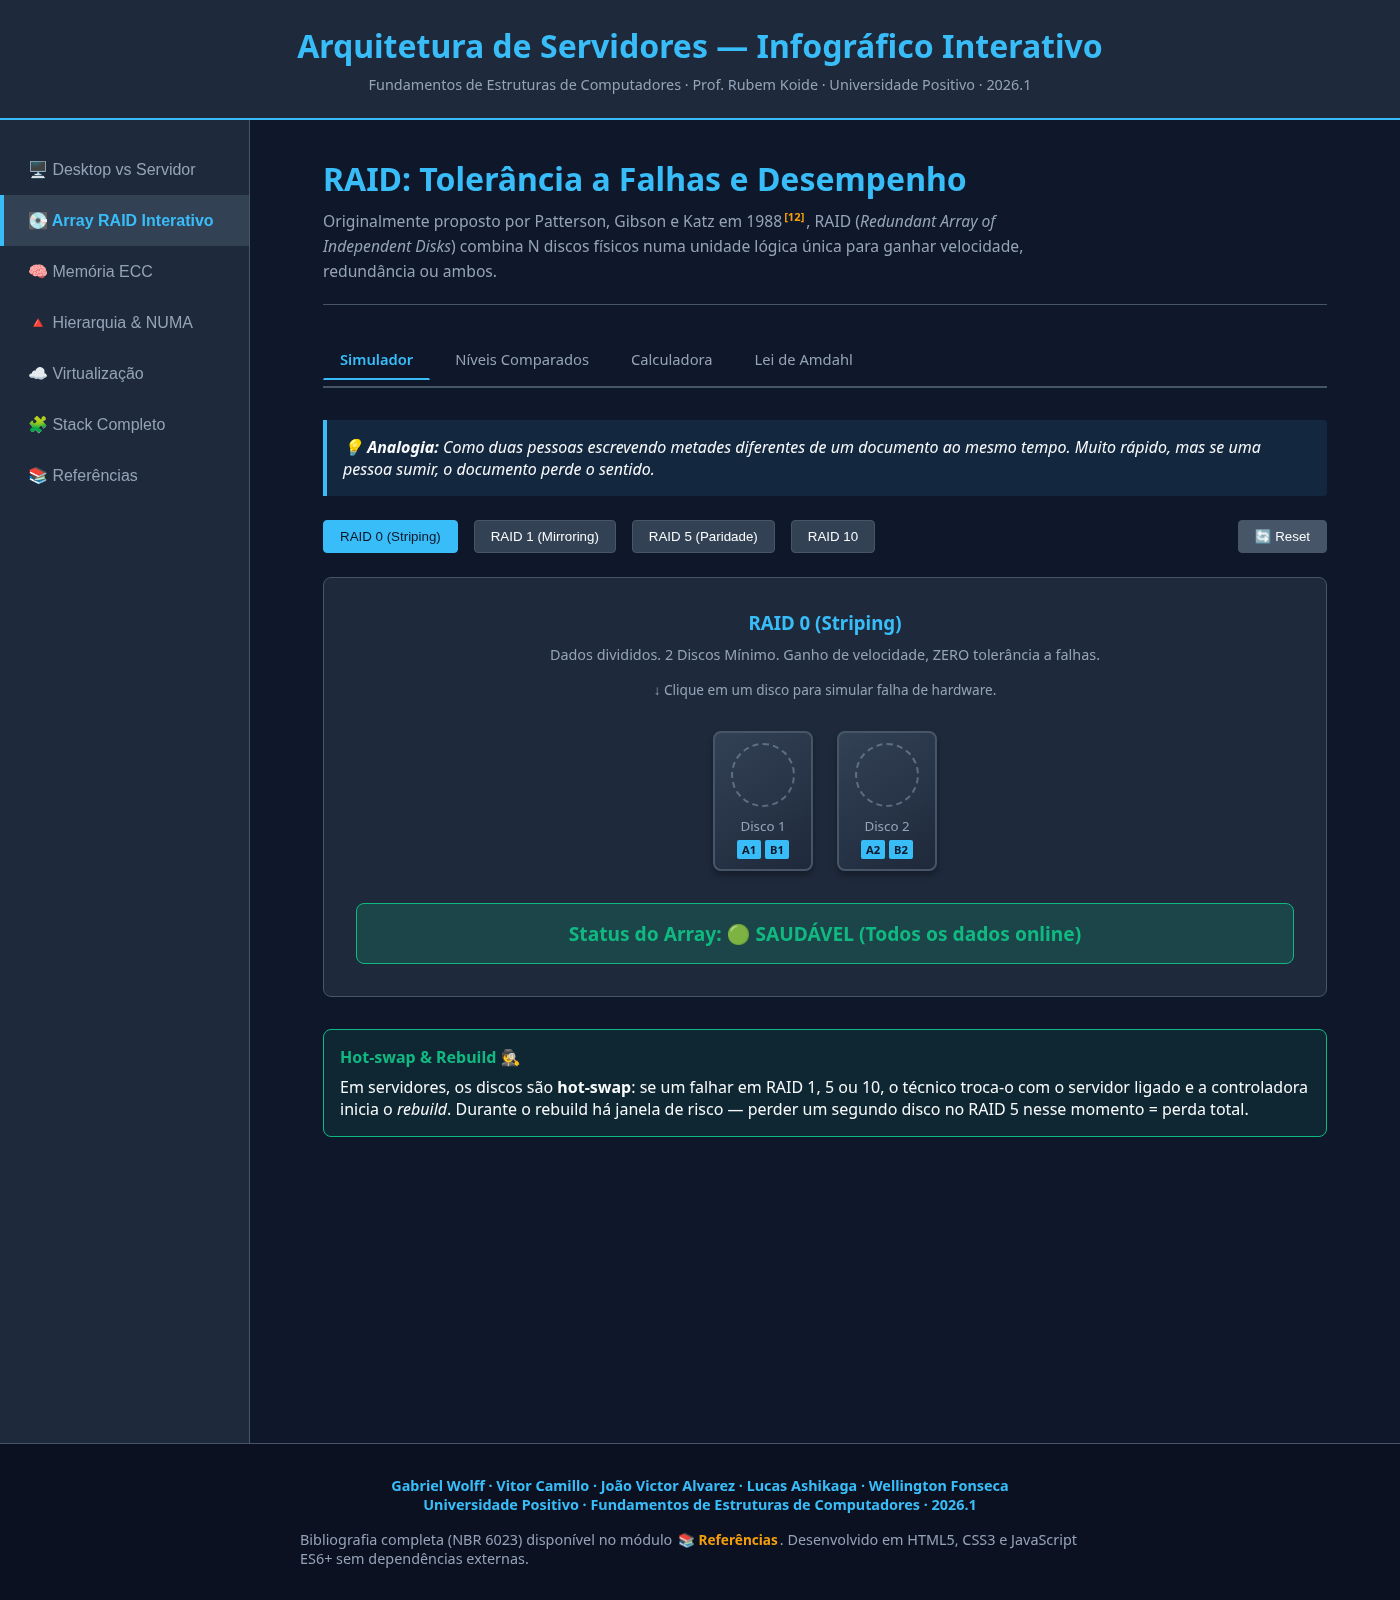
\includegraphics[width=0.95\textwidth]{figuras/mod2.png}
\caption{Módulo 2 --- RAID com simulador de falha.}
\label{fig:mod2}
\end{figure}

Distribuído em quatro sub-abas:

\begin{description}
    \item[Simulador] reproduz a versão original do módulo --- o
          aluno seleciona o nível \textsc{raid} (0, 1, 5 ou 10), o
          sistema desenha os discos e calcula em tempo real o
          impacto de cliques sucessivos (falhas) sobre o
          \emph{status} do \emph{array}.
    \item[Níveis Comparados] tabela com seis níveis (0, 1, 5, 6, 10,
          50) detalhando capacidade útil, tolerância e penalidade de
          escrita, mais a fórmula explícita de paridade
          $P = A \oplus B \oplus C$.
    \item[Calculadora] formulário onde o usuário escolhe nível,
          número de discos, capacidade individual e \textsc{iops} por
          disco; o sistema computa capacidade útil, eficiência de
          espaço, discos toleráveis e \textsc{iops} de leitura/escrita
          considerando a penalidade do nível selecionado.
    \item[Lei de Amdahl] aplicação numérica do
          Capítulo~\ref{cap:referencial}, com simulador interativo
          (\emph{slider} de fração paralelizável $P$ e número de
          discos $N$) que recalcula o \emph{speedup} efetivo e o
          teto teórico em tempo real.
\end{description}

\subsection{Lógica do simulador de falhas}

O estado do \emph{array} é mantido num vetor JavaScript
\texttt{raidState}; cada elemento descreve o ID do disco e se ele
está em falha. A função \texttt{updateRaidStatus()} contém o
\texttt{switch} que codifica o comportamento esperado de cada nível
sob diferentes contagens de falhas (Listagem~\ref{lst:raidstatus}).

\begin{lstlisting}[language=JavaScript,label=lst:raidstatus,caption=Trecho da lógica de status do RAID]
switch(currentRaid) {
    case 0:
        statusClass = 'status-fail';
        statusStr   = 'PERDA TOTAL! RAID 0 não tolera falhas.';
        break;
    case 1:
        if (failedCount === 1) { statusClass = 'status-warn';
            statusStr = 'DEGRADADO! Operando só pelo espelho.'; }
        else { statusClass = 'status-fail';
            statusStr = 'FALHA CRITICA! Ambos espelhos perdidos.'; }
        break;
    case 5:
        if (failedCount === 1) { statusClass = 'status-warn';
            statusStr = 'DEGRADADO! Recalculando paridade.'; }
        else { statusClass = 'status-fail';
            statusStr = 'RAID 5 só tolera 1 falha.'; }
        break;
    /* ... RAID 10 omitido por brevidade ... */
}
\end{lstlisting}

\subsection{Calculadora de IOPS}

A fórmula adotada para a penalidade de escrita segue a literatura
padrão de armazenamento empresarial:

\begin{equation}
\mathrm{IOPS}_{\text{escrita}} = \frac{N \cdot \mathrm{IOPS}_{\text{disco}}}{\text{penalty}}
\quad \text{com penalty} \in \{1, 2, 4, 6, 2\}
\end{equation}

para os níveis 0, 1, 5, 6, 10 respectivamente. Isso reproduz o
conhecido ``RAID~5 \emph{write penalty}'' de fator 4.

\section{Módulo 3 --- Memória ECC e Hamming \textsc{secded}}
\label{sec:mod3}

\begin{figure}[h!]
\centering
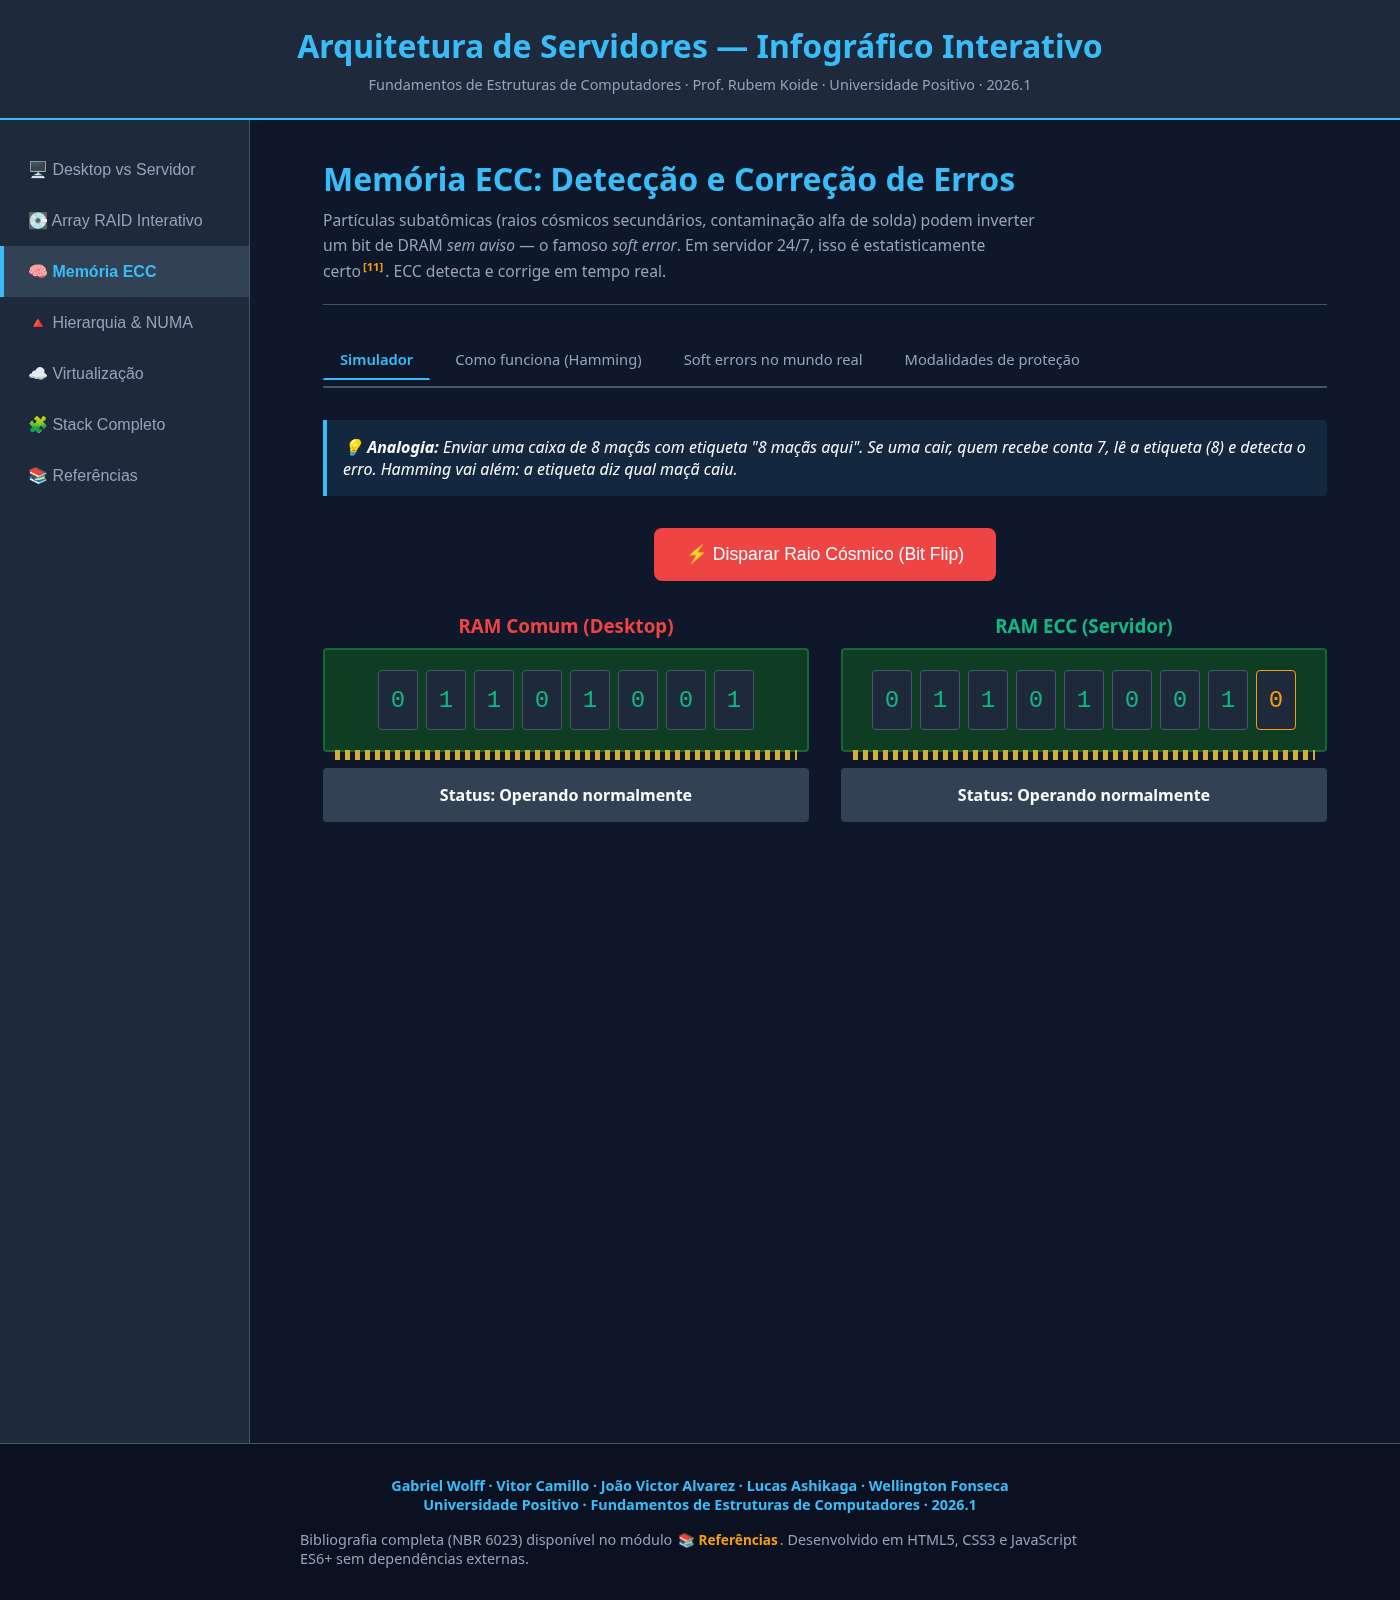
\includegraphics[width=0.95\textwidth]{figuras/mod3.png}
\caption{Módulo 3 --- Memória ECC: simulador de bit flip.}
\label{fig:mod3}
\end{figure}

Quatro sub-abas:

\begin{description}
    \item[Simulador] herda a animação original de raio cósmico,
          comparando lado-a-lado RAM comum e RAM \textsc{ecc}.
    \item[Como funciona (Hamming)] mostra os 12 bits da palavra
          Hamming(12,8) com correção de erro único (SEC): quatro
          paridades $P_1, P_2, P_4, P_8$ nas posições $2^k$, oito
          bits de dado, e a extensão para (13,8) (\textsc{secded})
          via bit de paridade global.
    \item[Soft errors no mundo real] expõe os números do estudo de
          Schroeder \textit{et al.}~\cite{schroeder2009} ---
          25\,000 a 70\,000 \textsc{fit} por \textsc{mb}it,
          mais de 8\,\% dos \textsc{dimm}s afetados por ano --- e
          cita o caso da eleição federal belga em Schaerbeek
          (2003), em que a candidata Maria Vindevoghel recebeu
          4\,096 votos extras por inversão de um único bit na
          posição 13 do contador, atribuída a um \emph{single-event
          upset} (hipótese provável, nunca comprovada definitivamente).
    \item[Modalidades de proteção] tabela comparando paridade
          simples, \textsc{secded}, Chipkill/\textsc{sddc} e
          \textsc{ddr5} \emph{on-die} \textsc{ecc}.
\end{description}

\subsection{Cálculo do síndrome}

Com 4 bits de paridade, a representação binária do \emph{síndrome}
recalculado na leitura tem 16 valores possíveis; 0 indica ausência
de erro, e os demais indicam exatamente a posição do bit
corrompido. Por exemplo: paridades $(s_3, s_2, s_1, s_0) = (0,1,0,1)$
$\Rightarrow$ posição decimal 5 $\Rightarrow$ corrupção em $D_2$
(o segundo bit de dado, na posição 5 do layout Hamming).

\section{Módulo 4 --- Hierarquia, Cache e NUMA}
\label{sec:mod4}

\begin{figure}[h!]
\centering
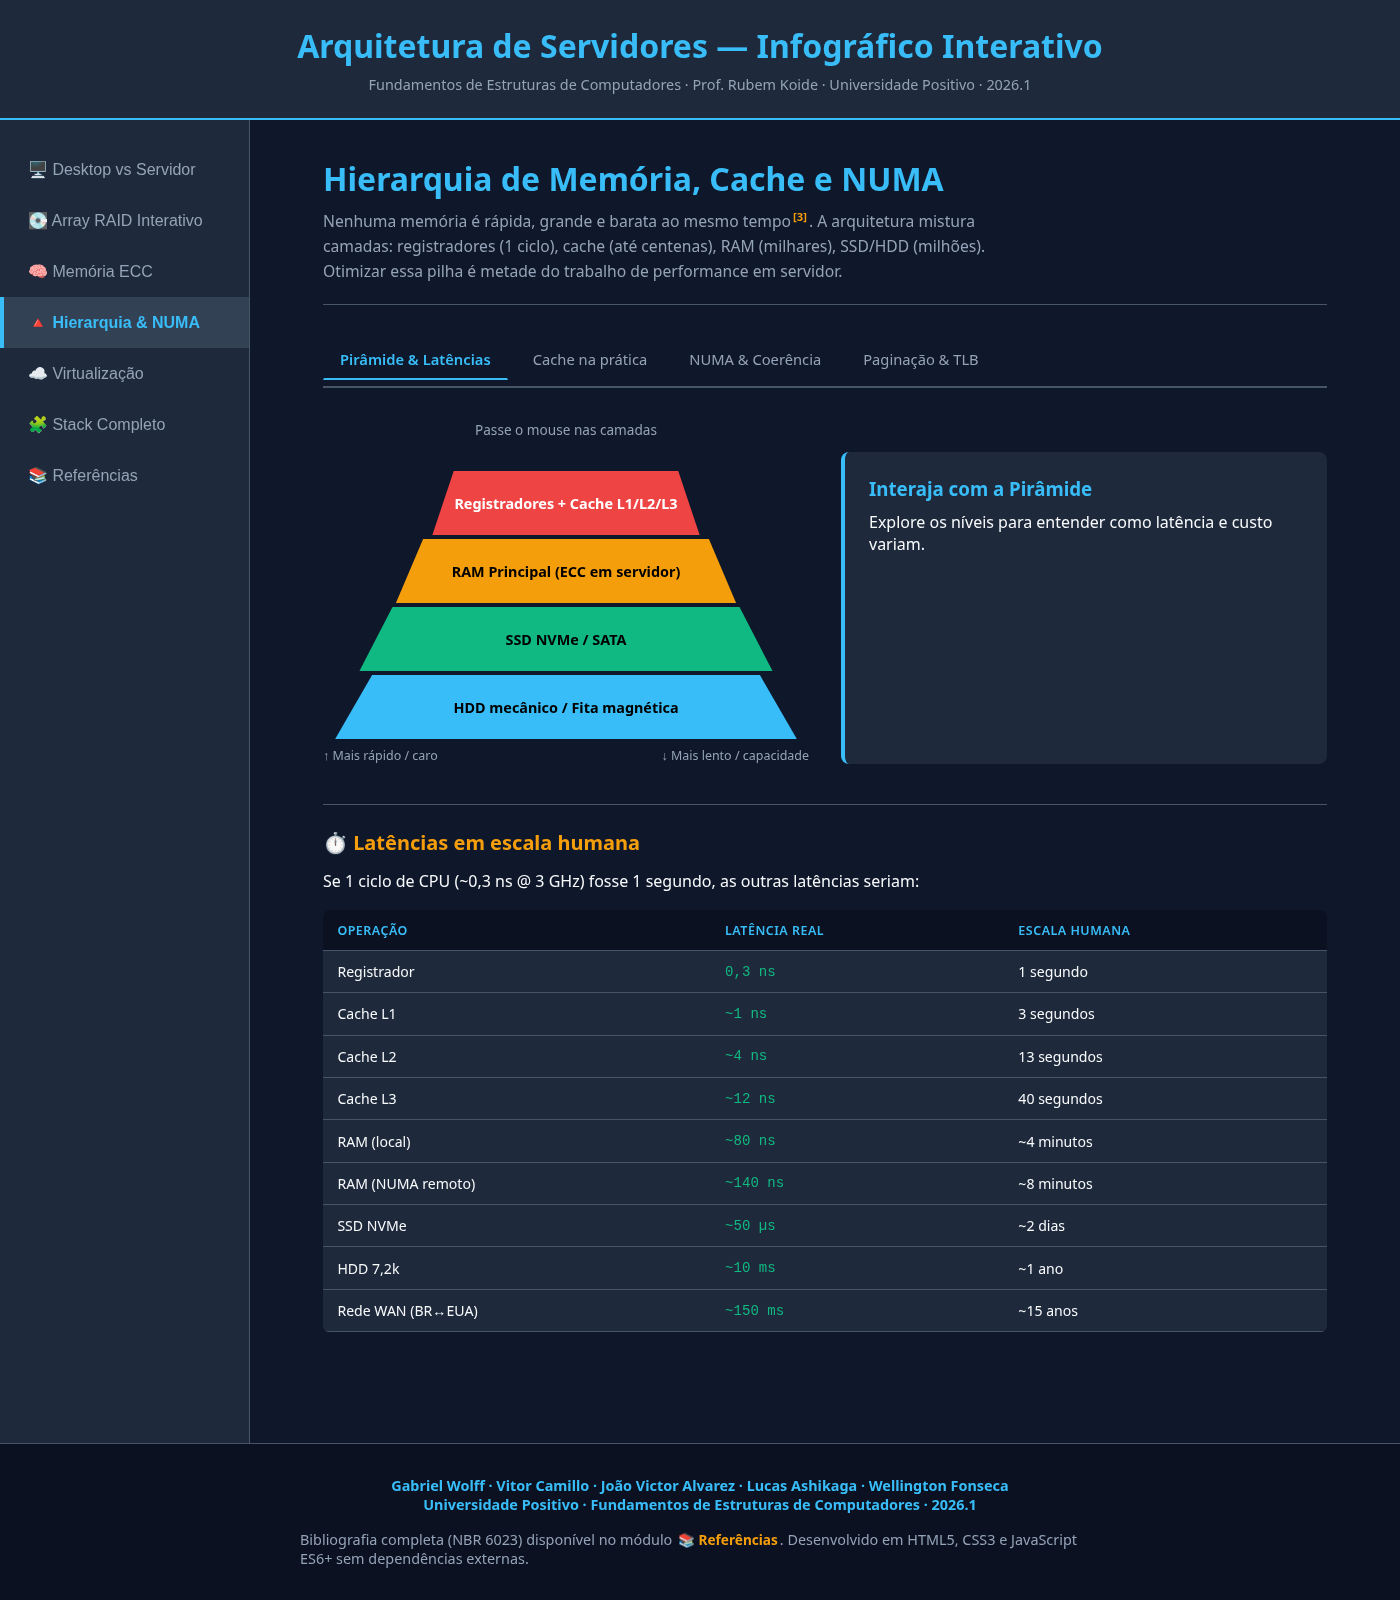
\includegraphics[width=0.95\textwidth]{figuras/mod4.png}
\caption{Módulo 4 --- Pirâmide de memória com latências em escala humana.}
\label{fig:mod4}
\end{figure}

Quatro sub-abas:

\begin{description}
    \item[Pirâmide \& Latências] versão original da pirâmide
          interativa com hover, complementada por uma tabela que
          escalona as latências para a referência humana (se 1
          ciclo de CPU equivalesse a 1 segundo, um acesso à RAM
          remota NUMA equivaleria a 8 minutos).
    \item[Cache na prática] tabela com a hierarquia real de um Intel
          Core i7-5960X (Tabela~\ref{tab:cache-i7}) e simulador de
          \emph{cache hit/miss} animado.
    \item[NUMA \& Coerência] diagrama \emph{dual-socket} com
          latência local (80\,\textsc{ns}) versus remota
          (140\,\textsc{ns}), e tabela explicando os 4 estados do
          protocolo \textsc{mesi}.
    \item[Paginação \& TLB] páginas de 4\,\textsc{kb} \emph{vs.}
          \textit{huge pages} de 2\,\textsc{mb}, \textit{page walk}
          em 4 níveis no x86-64, fórmula
          $t_{\text{acesso}} = t_{\text{tlb}} + (\text{taxa\_miss} \cdot t_{\text{pagewalk}})$.
\end{description}

\begin{table}[h!]
\centering
\caption{Cache do Intel Core i7-5960X (8 cores, Haswell-E)}
\label{tab:cache-i7}
\begin{tabular}{lrlrl}
\toprule
\textbf{Nível} & \textbf{Tamanho} & \textbf{Assoc.} &
\textbf{Latência} & \textbf{Escopo} \\
\midrule
L1d   & 32 KB  & 8-way  & 4 ciclos  & Por core \\
L1i   & 32 KB  & 8-way  & 4 ciclos  & Por core \\
L2    & 256 KB & 8-way  & 12 ciclos & Por core \\
L3    & 20 MB  & 20-way & 38 ciclos & 8 cores \\
\bottomrule
\end{tabular}
\end{table}

\subsection{Simulador de acesso à cache}

Implementa probabilidades empíricas típicas: 92\,\% de \textit{hit}
em L1, 6\,\% em L2, 1,5\,\% em L3 e 0,5\,\% \textit{miss} até a RAM.
A cada clique no botão ``Simular acesso'', a função
\texttt{simulateCacheAccess()} sorteia o resultado e anima a
travessia da pirâmide marcando \emph{miss} em cinza e \emph{hit} em
verde, exibindo o custo em ciclos do nível atingido.

\section{Módulo 5 --- Virtualização}
\label{sec:mod5}

\begin{figure}[h!]
\centering
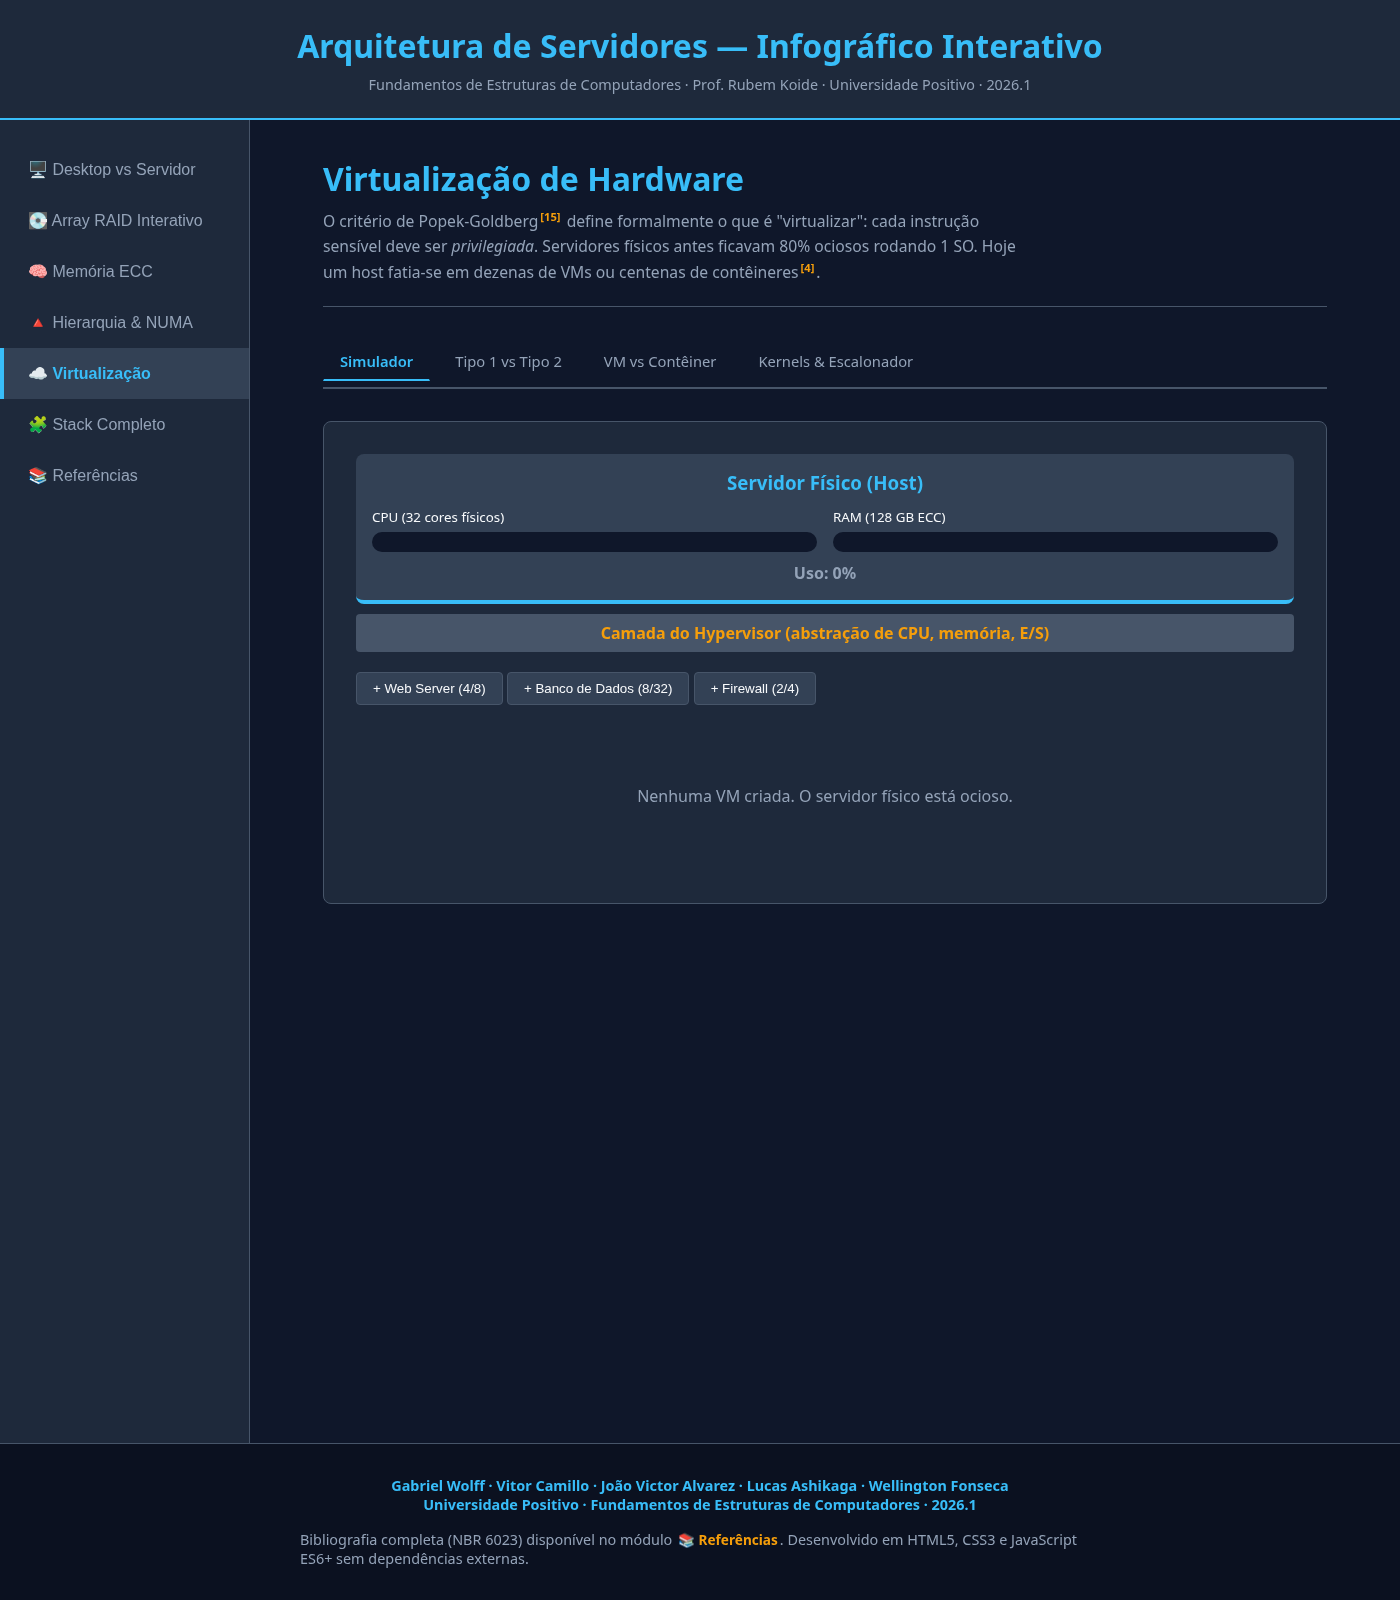
\includegraphics[width=0.95\textwidth]{figuras/mod5.png}
\caption{Módulo 5 --- Alocador de máquinas virtuais sobre o \emph{host} físico.}
\label{fig:mod5}
\end{figure}

Quatro sub-abas:

\begin{description}
    \item[Simulador] o alocador de VMs original, que limita a soma
          de v\textsc{cpu}s e RAM ao máximo físico (32 cores /
          128\,\textsc{gb}) e visualmente preenche barras de
          recurso, vermelha se acima de 80\,\%.
    \item[Tipo 1 \textit{vs.}\ Tipo 2] tabela taxonômica + diagrama
          dos anéis de proteção x86, incluindo o
          \textsc{vmx} \emph{root} (Ring~$-1$) introduzido por
          \textsc{vt-x}/AMD-V, e curiosidade sobre \textsc{wsl}~2
          como caso de virtualização leve.
    \item[VM \textit{vs.}\ Contêiner] tabela comparando granularidade,
          \emph{boot time}, \textit{footprint} e densidade, mais um
          trecho de código Linux mostrando criação manual de
          contêiner com \texttt{unshare} + \texttt{cgroups}.
    \item[Kernels \& Escalonador] comparação Windows NT (híbrido)
          \emph{vs.}\ Linux (monolítico modular), com diagrama da
          árvore rubro-negra usada pelo \textsc{cfs}.
\end{description}

\section{Módulo 6 --- \emph{Stack} Completo}
\label{sec:mod6}

\begin{figure}[h!]
\centering
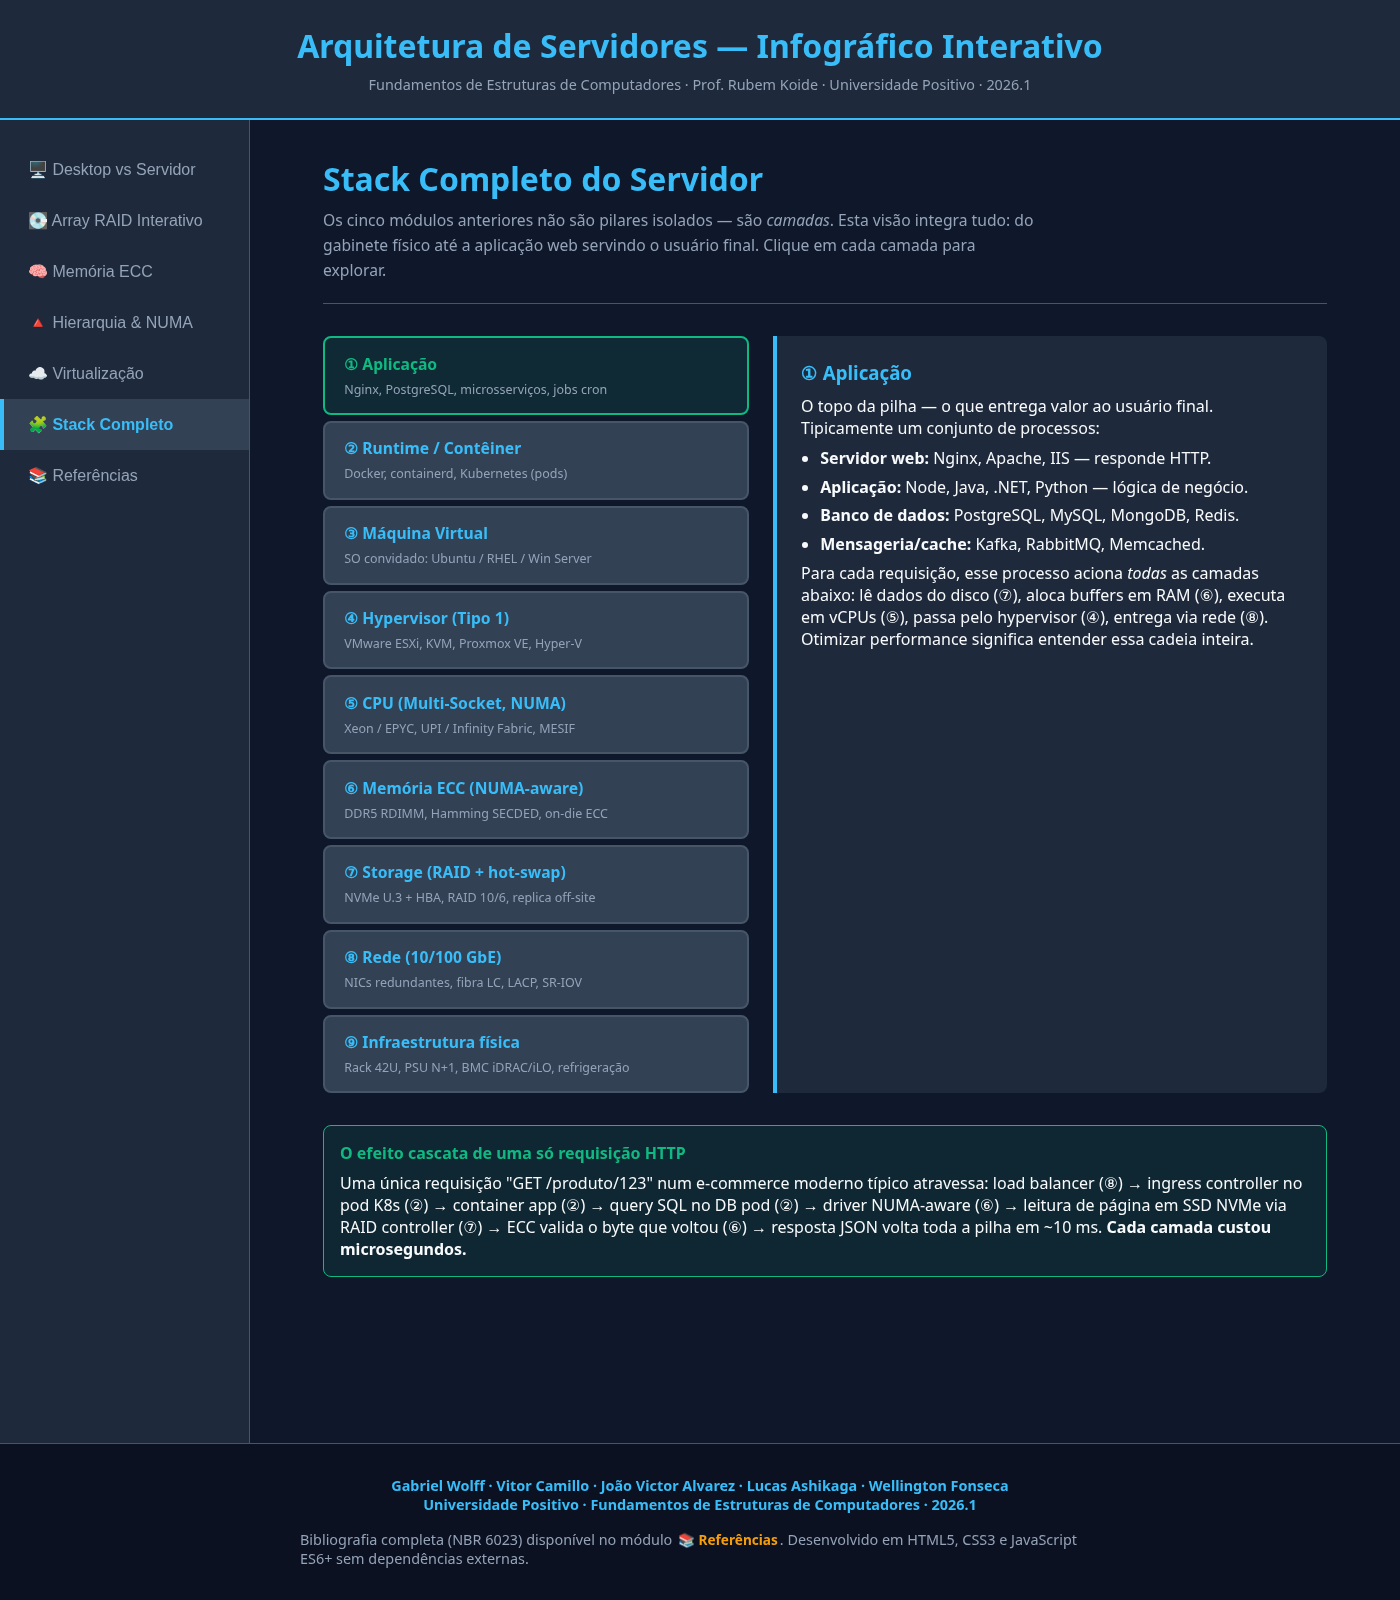
\includegraphics[width=0.95\textwidth]{figuras/mod6.png}
\caption{Módulo 6 --- \emph{Stack} integrado do servidor de produção.}
\label{fig:mod6}
\end{figure}

Este módulo \textbf{não tem sub-abas}: é uma síntese visual integrando
todas as camadas anteriores num único diagrama vertical com 9
camadas clicáveis, do nível físico (PSU, BMC, rack) até a aplicação
no topo (Nginx, PostgreSQL, microsserviços). Ao clicar em cada
camada, o painel à direita exibe seu detalhamento técnico --- com
referências cruzadas aos módulos anteriores.

\subsection{Modelo de dados das camadas}

A informação de cada camada é mantida num objeto JavaScript
\texttt{stackData}, conforme o trecho da Listagem~\ref{lst:stackdata}.

\begin{lstlisting}[language=JavaScript,label=lst:stackdata,caption=Estrutura de dados das camadas do stack]
const stackData = {
    cpu: {
        title: 'CPU (Multi-Socket, NUMA)',
        body:  '<p>Em servidor, 2-8 sockets físicos compartilham ' +
               'a memória via UPI (Intel) ou Infinity Fabric (AMD)' +
               ', com protocolo MESIF/MOESI para coerência.</p>' +
               '<ul><li>Xeon Scalable / EPYC: 16-128 cores/socket</li>' +
               '<li>Hyperthreading: 2 threads lógicos por core físico</li>' +
               '<li>NUMA-aware: scheduler mantém threads próximas à RAM</li>' +
               '</ul>'
    },
    /* ... outras 8 camadas omitidas por brevidade ... */
};
\end{lstlisting}

A função \texttt{showStackDetail(key, el)} troca o painel da direita
para o conteúdo da camada selecionada, mantendo o histórico de
seleção via classe CSS \texttt{.active}.

\section{Módulo de Referências}
\label{sec:mod-ref}

Um sétimo item de navegação --- \textbf{Referências} --- expõe a
lista bibliográfica completa formatada conforme \textsc{abnt}
\textsc{nbr} 6023:2018. Cada citação inline nos módulos é um link
ativo: ao clicar em \texttt{[11]}, por exemplo, o usuário é
transportado para a aba de referências e a entrada $11$ é
destacada em laranja por 2,5 segundos --- comportamento
implementado em \texttt{goToRef(n)}
(Listagem~\ref{lst:gotoref}).

\begin{lstlisting}[language=JavaScript,label=lst:gotoref,caption=Função de navegação para referência citada]
function goToRef(n) {
    showModule('modRef', null);
    setTimeout(() => {
        const target = document.getElementById('ref-' + n);
        if (!target) return;
        target.scrollIntoView({ behavior: 'smooth', block: 'center' });
        target.classList.add('highlight');
        setTimeout(() => target.classList.remove('highlight'), 2500);
    }, 200);
}
\end{lstlisting}

\section{Resultado consolidado}

O artefato final possui:

\begin{itemize}
    \item 6 módulos temáticos + 1 índice de referências;
    \item 21 sub-abas no total (média de 3,5 por módulo);
    \item 17 referências bibliográficas \textsc{abnt} clicáveis;
    \item 11 tabelas técnicas com dados quantitativos;
    \item 8 simulações interativas em JavaScript;
    \item aproximadamente 2\,500 linhas em arquivo HTML único;
    \item \emph{zero} dependências externas, executável \textit{offline}.
\end{itemize}

O salto de profundidade entre as duas iterações pode ser quantificado
de forma simples: a primeira versão do código tinha 1\,060 linhas e
3 referências bibliográficas; a segunda chega a 2\,554 linhas e
17 referências, com adição de todas as fórmulas, tabelas e
simuladores listados acima.

\chapter{Conclusão}
\label{cap:conclusao}

O presente trabalho desenvolveu um infográfico interativo sobre
arquitetura de servidores, materializando, em forma de artefato
didático executável em navegador, o conteúdo das aulas 6 a 12 da
disciplina de Fundamentos de Estruturas de Computadores.

O processo passou por duas iterações. A primeira versão estabeleceu
o esqueleto visual e a interatividade básica, mas foi avaliada pelo
orientador como insuficiente em profundidade técnica. A segunda
iteração --- a que este relatório descreve --- refatorou cada
módulo para incorporar tabelas comparativas com números reais
(barramentos, latências, capacidades), fórmulas explícitas (Amdahl,
paridade XOR, síndrome de Hamming), \emph{specs} de processadores
reais (Intel Core i7-5960X, Xeon Scalable, EPYC, NVIDIA Grace
Hopper), bibliografia formal \textsc{abnt} \textsc{nbr 6023}
acessível diretamente do infográfico via citações clicáveis, e um
sexto módulo integrador (\emph{stack} completo) que sintetiza os
cinco anteriores numa única visão.

\section{Aderência aos objetivos}

Confrontados com os objetivos específicos enunciados na
Seção~1.2, observamos:

\begin{itemize}
    \item \textbf{Comparativo Desktop \textit{vs.}\ Servidor}: atendido
          com a sub-aba ``Visão Geral'' e complementado com três
          aprofundamentos (Interconexão CPU, Barramentos de E/S,
          IA \& HPC) ausentes na primeira versão.
    \item \textbf{Simulação de RAID e cálculo quantitativo}: atendido
          com o simulador original mais uma calculadora de \textsc{iops}
          e capacidade útil e a aplicação numérica da Lei de Amdahl
          ao exemplo do servidor \textsc{www}.
    \item \textbf{Visualização do código de Hamming}: atendido com a
          sub-aba ``Como funciona'', que expõe os 12 bits da palavra
          Hamming(12,8) e a tabela de cobertura dos bits de paridade.
    \item \textbf{Hierarquia com latências em escala humana}: atendido
          com tabela conversora (ciclo de CPU $\to$ 1 segundo) e
          simulador de \textit{cache hit/miss} animado.
    \item \textbf{Virtualização Tipo 1 \textit{vs.}\ Tipo 2}:
          atendido com taxonomia, anéis de proteção x86 (Ring 0 a
          Ring~$-1$) e comparação dedicada VM \textit{vs.}\ contêiner.
    \item \textbf{Integração final}: atendido com o Módulo 6
          (\emph{stack} completo), inexistente na primeira versão.
\end{itemize}

\section{Limitações}

Algumas escolhas conscientes restringem o alcance do artefato:

\begin{enumerate}
    \item Por se tratar de aplicação \emph{client-side} sem
          \emph{back-end}, nenhum dos simuladores executa medições
          reais de hardware; todos os números (\textsc{iops},
          latência, \emph{speedup}) são calculados via fórmulas
          determinísticas com parâmetros tabulares ou via amostragem
          de uma distribuição empírica.
    \item A análise da Lei de Amdahl considera apenas o cenário
          ideal de paralelização homogênea entre discos, ignorando
          contenção de barramento, \emph{cache pollution} e custo
          do controlador \textsc{raid}.
    \item A visualização do escalonador \textsc{cfs} é estática
          (árvore exemplificativa); não há simulador de inserção e
          remoção de \emph{tasks} ao longo do tempo.
    \item O suporte mobile é funcional (\emph{media queries} em três
          \emph{breakpoints}), mas tabelas extensas precisam de
          rolagem horizontal em telas estreitas.
\end{enumerate}

\section{Trabalhos futuros}

\begin{itemize}
    \item \textbf{Animar a coerência \textsc{mesi/mesif}}: implementar
          um simulador onde dois \emph{cores} disputam uma linha de
          cache e o usuário acompanha as transições de estado.
    \item \textbf{Visualização do \emph{page walk}}: animar a
          tradução de um endereço virtual nos 4 níveis da
          paginação x86-64, com e sem \textit{TLB hit}.
    \item \textbf{Integração com benchmarks reais}: incorporar
          dados de \texttt{fio}, \texttt{stress-ng} e
          \texttt{lmbench} para ancorar os valores teóricos em
          medições reproduzíveis.
    \item \textbf{Tradução para o inglês}: o infográfico tem
          potencial além do escopo da disciplina --- com tradução,
          poderia servir como recurso aberto (CC-BY) para outras
          turmas de Arquitetura de Computadores.
    \item \textbf{Acessibilidade}: auditar para conformidade
          \textsc{wcag} 2.1 \textsc{aa}, garantindo navegação por
          teclado e leitor de tela em todos os simuladores.
\end{itemize}

\section{Considerações finais}

O salto de profundidade entre as duas iterações --- de 1\,060 para
2\,554 linhas de código, de 3 para 17 referências bibliográficas,
de zero para 11 tabelas quantitativas e de 5 para 8 simuladores
interativos --- ilustra que a profundidade técnica de um artefato
didático é fundamentalmente uma decisão \emph{de conteúdo}, não de
arquitetura de software. Manter o projeto em um único arquivo HTML
sem dependências facilitou justamente esse aprofundamento: toda a
energia da segunda iteração pôde ser direcionada para a leitura
crítica do material das aulas e para a tradução dos conceitos em
visualizações executáveis, sem ser desperdiçada em configuração de
\emph{build tools} ou gerenciamento de pacotes.

O resultado é um artefato que, esperamos, faça jus à
crítica original do orientador e demonstre, de forma navegável e
auto-contida, por que um servidor é mais do que ``um computador
maior'' --- e quais subsistemas precisam estar bem compreendidos
para projetá-lo, operá-lo ou estudá-lo.


% ==================== ELEMENTOS PÓS-TEXTUAIS ====================
\postextual

\bibliography{references}

\begin{anexosenv}
\partanexos
\chapter{Código-fonte do infográfico}
\label{anx:codigo}

\section{Repositório completo}

O código-fonte completo do infográfico, com histórico de \emph{commits}
e \texttt{README} de instruções, encontra-se em:

\begin{center}
\fbox{\parbox{0.9\textwidth}{\centering\vspace{6pt}
\large \url{https://github.com/glkwolff/Projeto-Estruturas-de-computadores}
\vspace{6pt}}}
\end{center}

A reprodução integral neste anexo é impraticável: o arquivo
\texttt{projeto.html} ultrapassa 2\,500 linhas e o critério de
entrega prevê justamente que, em código longo, se descreva o link
no relatório. As listagens a seguir trazem apenas trechos críticos
ilustrativos.

\section{Estrutura do arquivo único}

\begin{lstlisting}[language=HTML,caption=Esqueleto geral do projeto.html]
<!DOCTYPE html>
<html lang="pt-BR">
<head>
  <meta charset="UTF-8">
  <title>Arquitetura de Servidores - Infográfico Interativo</title>
  <style>
    /* ~600 linhas de CSS:
       custom properties, layout flex/grid, tabelas, animações */
  </style>
</head>
<body>
  <header> ... </header>
  <div class="container">
    <nav>  <!-- 7 botões de navegação --> </nav>
    <main>
      <section id="mod1"  class="module active"> <!-- Módulo 1 --> </section>
      <section id="mod2"  class="module">        <!-- Módulo 2 --> </section>
      <section id="mod3"  class="module">        <!-- Módulo 3 --> </section>
      <section id="mod4"  class="module">        <!-- Módulo 4 --> </section>
      <section id="mod5"  class="module">        <!-- Módulo 5 --> </section>
      <section id="mod6"  class="module">        <!-- Módulo 6 --> </section>
      <section id="modRef" class="module">       <!-- Referências --> </section>
    </main>
  </div>
  <footer> ... </footer>
  <script>
    /* ~600 linhas de JavaScript:
       navegação, sub-abas, simulações por módulo */
  </script>
</body>
</html>
\end{lstlisting}

\section{Função de navegação por sub-abas}

\begin{lstlisting}[language=JavaScript,caption=Implementação das sub-abas dentro de cada módulo]
function showPanel(modId, panelId, element) {
    const root = document.getElementById(modId);
    if (!root) return;
    root.querySelectorAll('.mod-panel').forEach(p =>
        p.classList.remove('active'));
    root.querySelectorAll('.mod-tab').forEach(t =>
        t.classList.remove('active'));
    const panel = document.getElementById(panelId);
    if (panel) panel.classList.add('active');
    if (element) element.classList.add('active');
}
\end{lstlisting}

\section{Cálculo do simulador RAID}

\begin{lstlisting}[language=JavaScript,caption=Calculadora de IOPS e capacidade útil]
function calcRaid() {
    const level = parseInt(document.getElementById('rc-level').value);
    let   n     = parseInt(document.getElementById('rc-disks').value);
    const cap   = parseFloat(document.getElementById('rc-cap').value);
    const iops  = parseInt(document.getElementById('rc-iops').value);

    const mins = { 0: 2, 1: 2, 5: 3, 6: 4, 10: 4 };
    if (n < mins[level]) n = mins[level];
    if (level === 10 && n % 2 !== 0) n -= 1;

    let useful, tolerable, penalty;
    switch (level) {
        case 0:  useful = n * cap;       tolerable = 0;     penalty = 1; break;
        case 1:  useful = cap;           tolerable = n-1;   penalty = 2; break;
        case 5:  useful = (n-1) * cap;   tolerable = 1;     penalty = 4; break;
        case 6:  useful = (n-2) * cap;   tolerable = 2;     penalty = 6; break;
        case 10: useful = (n/2) * cap;   tolerable = n/2;   penalty = 2; break;
    }
    const iopsR = n * iops;
    const iopsW = Math.round((n * iops) / penalty);
    /* ... atualização da DOM omitida ... */
}
\end{lstlisting}

\section{Aplicação da Lei de Amdahl}

\begin{lstlisting}[language=JavaScript,caption=Simulador interativo da Lei de Amdahl]
function updateAmdahl() {
    const P = parseFloat(document.getElementById('am-p').value);
    const N = parseInt  (document.getElementById('am-n').value);

    const speedup = 1 / ((1 - P) + (P / N));
    const ceiling = P === 1 ? Infinity : 1 / (1 - P);
    const util    = ceiling === Infinity ? '—'
                  : ((speedup / ceiling) * 100).toFixed(0) + '%';

    document.getElementById('am-out-speedup').innerText = speedup.toFixed(2) + 'x';
    document.getElementById('am-out-cap').innerText     = ceiling === Infinity
                                                        ? 'inf'
                                                        : ceiling.toFixed(2) + 'x';
    document.getElementById('am-out-util').innerText    = util;
}
\end{lstlisting}

\section{Simulador de \textit{cache hit/miss}}

\begin{lstlisting}[language=JavaScript,caption=Animação de travessia na hierarquia de memória]
function simulateCacheAccess() {
    const r = Math.random();
    let hitAt, cycles;
    if      (r < 0.92)  { hitAt = 'l1';  cycles = 4;   }
    else if (r < 0.98)  { hitAt = 'l2';  cycles = 12;  }
    else if (r < 0.995) { hitAt = 'l3';  cycles = 38;  }
    else                { hitAt = 'ram'; cycles = 250; }

    const order = ['l1', 'l2', 'l3', 'ram'];
    const hitIndex = order.indexOf(hitAt);
    order.forEach((lvl, i) => {
        setTimeout(() => {
            const el = document.querySelector(
                `#cache-trace .cache-level[data-cl="${lvl}"]`);
            if (i <  hitIndex) el.classList.add('miss');
            if (i === hitIndex) el.classList.add('hit');
        }, i * 250);
    });
}
\end{lstlisting}

\section{Navegação para referência citada}

\begin{lstlisting}[language=JavaScript,caption=Função que vincula cita inline ao item bibliográfico]
function goToRef(n) {
    showModule('modRef', null);
    setTimeout(() => {
        const target = document.getElementById('ref-' + n);
        if (!target) return;
        target.scrollIntoView({ behavior: 'smooth', block: 'center' });
        target.classList.add('highlight');
        setTimeout(() => target.classList.remove('highlight'), 2500);
    }, 200);
}
\end{lstlisting}

\section{Como executar localmente}

\begin{enumerate}
    \item Clonar o repositório: \\
          \texttt{git clone https://github.com/glkwolff/Projeto-Estruturas-de-computadores}
    \item Abrir o arquivo \texttt{projeto.html} em qualquer navegador
          moderno (Chrome 130+, Firefox 130+, Edge 130+).
    \item Nenhuma instalação, servidor local ou conexão de internet é
          necessária.
\end{enumerate}

\end{anexosenv}

\end{document}
